\documentclass[a4paper,11pt,twoside]{memoir}
\setcounter{secnumdepth}{2}
\let\STARTCODE\relax 
\let\STOPCODE\relax 
\STARTCODE
\usepackage{color,calc,graphicx,soul}
\definecolor{nicered}{rgb}{.647,.129,.149} \makeatletter
\newlength\dlf@normtxtw \setlength\dlf@normtxtw{\textwidth}
\def\myhelvetfont{\def\sfdefault{mdput}} \newsavebox{\feline@chapter}
\newcommand\feline@chapter@marker[1][4cm]{
  \sbox\feline@chapter{
    \resizebox{!}{#1}{\fboxsep=1pt
      \colorbox{nicered}{\color{white}\bfseries\sffamily\thechapter}
    }}
  \rotatebox{90}{
    \resizebox{
      \heightof{\usebox{\feline@chapter}}+\depthof{\usebox{\feline@chapter}}}
    {!}{\scshape\so\@chapapp}}\quad
  \raisebox{\depthof{\usebox{\feline@chapter}}}{\usebox{\feline@chapter}}
} \newcommand\feline@chm[1][4cm]{
  \sbox\feline@chapter{\feline@chapter@marker[#1]}
  \makebox[0pt][l]{
    \makebox[1cm][r]{\usebox\feline@chapter}
  }} \makechapterstyle{daleif1}{
  \setlength{\afterchapskip}{10pt}
  \renewcommand{\insertchapterspace}{}
  \renewcommand\chapnamefont{\normalfont\Large\scshape\raggedleft\so}
  \renewcommand\chaptitlefont{\normalfont\huge\bfseries\scshape\color{nicered}}
  \renewcommand\chapternamenum{} 
  \renewcommand\printchaptername{}
  \renewcommand\printchapternum{\vspace{-1.8cm}\null\hfill\feline@chm[2.5cm]\par}
  \renewcommand\afterchapternum{\par\vskip\midchapskip}
  \renewcommand\printchaptertitle[1]{\chaptitlefont\raggedleft
    ##1\par}
  \renewcommand\printchapternonum{\vspace{0.2cm}}
}
\makeatother
\chapterstyle{daleif1}
\STOPCODE
\usepackage[utf8x]{inputenc}
\usepackage[T1]{fontenc}
\usepackage[english, french]{babel}
\usepackage{lipsum}
\usepackage{lmodern}
\rmfamily
\DeclareFontShape{T1}{lmr}{b}{sc}{<->ssub*cmr/bx/sc}{}
\DeclareFontShape{T1}{lmr}{bx}{sc}{<->ssub*cmr/bx/sc}{}
\usepackage{epigraph}
\usepackage[french]{minitoc}
\setcounter{minitocdepth}{2}
\usepackage{soul}
\usepackage[pagebackref,colorlinks=true,citecolor=forestgreen,linkcolor=black,menucolor=alezan,urlcolor=prune]{hyperref}
\renewcommand*{\backref}[1]{}
\renewcommand*{\backrefalt}[4]{
\ifcase #1
-- Non cité.
\or
-- Cité page~#2.
\else
-- Cité pages~#2.
\fi}
\renewcommand*{\backrefsep}{, }
\renewcommand*{\backreftwosep}{ et~}
\renewcommand*{\backreflastsep}{ et~}
\usepackage{lingmacros}
\usepackage{fancybox}
\usepackage{pifont}
\usepackage{dsfont}
\def\sep{\begin{center}\begin{large}\ding{167}\end{large}\end{center}}
\renewcommand{\bibname}{Bibliographie}
\addto{\captionsenglish}{\renewcommand{\bibname}{Bibliographie}}
\addto{\captionsfrench}{\renewcommand{\listfigurename}{Liste des figures}}
\usepackage{newcent}
\usepackage{helvet}
\usepackage{color}
\usepackage{colortbl}
\usepackage{multirow}
\usepackage{longtable}
\newcommand{\withnofdp}[1]{{\NoAutoSpaceBeforeFDP #1}}
\usepackage{arydshln}
\usepackage{listings}
\lstset{
  language=XML, 
  basicstyle=\small,
  showspaces=false,
  showstringspaces=false,
  breaklines=true,
  breakatwhitespace=true,
  morecomment=[s]{<!--}{-->},
  alsoletter=.-,
  commentstyle=\itshape\color{gray},
  markfirstintag=true,
  string=[d]",
  keywords={correction},
  keywordstyle=\color{alizarine},
  stringstyle=\color{acier},
}
\usepackage{pgf,pgfarrows,pgfnodes}
\usepackage{tikz}
\usepackage{tikz-qtree}
\usepackage{tikz-dependency}
\usepackage{pgfplots}
\usetikzlibrary{mindmap,trees, backgrounds}
\usepackage{filecontents}
\usepackage{qtree}
\definecolor{acier}{HTML}{3A8EBA}
\definecolor{alezan}{HTML}{A76726}
\definecolor{alizarine}{HTML}{D90115}
\definecolor{amande}{HTML}{82C46C}
\definecolor{ambre}{HTML}{F0C300}
\definecolor{abricot}{HTML}{E67E30}
\definecolor{grey}{rgb}{0.9,0.9,0.9}
\definecolor{gris}{rgb}{0.1,0.1,0.1}
\definecolor{forestgreen}{rgb}{0.13,0.54,0.13}
\definecolor{dockerblue}{rgb}{0.11,0.56,0.98}
\definecolor{orange}{rgb}{0.64,0.16,0.16}
\definecolor{ocre}{HTML}{DFAF2C}
\definecolor{prune}{HTML}{811453}
\newcommand{\remCyril}[1]{\textcolor{dockerblue}{\emph{CG : #1}}}
\newcommand{\myex}[1]{\color{acier}{\emph{#1}}\color{black}}
\newcommand{\rg}[1]{\textsl{Remarque : #1}}
\def\euro{\mbox{\raisebox{.25ex}{{\it =}}\hspace{-.5em}{\sf C}}}
\newenvironment{changemargin}[2]{\begin{list}{}{
\setlength{\topsep}{0pt}
\setlength{\leftmargin}{0pt}
\setlength{\rightmargin}{0pt}
\setlength{\listparindent}{\parindent}
\setlength{\itemindent}{\parindent}
\setlength{\parsep}{0pt plus 1pt}
\addtolength{\leftmargin}{#1}
\addtolength{\rightmargin}{#2}
}\item }{\end{list}}
\usepackage{chngpage}
\usepackage{amssymb,amsmath,amsthm,amscd}
\usepackage{mathrsfs}
\usepackage{subfig}
\usepackage{tabularx}
\usepackage{calc}
\usepackage{graphicx}
\usepackage{hyperref}
\usepackage{makeidx}
\makeindex
\usepackage[french,intoc,refpage]{nomencl}
\renewcommand{\nomname}{Glossaire}
\renewcommand*{\pagedeclaration}[1]{\unskip\dotfill\hyperpage{#1}}
\makenomenclature
\newcommand{\nocontentsline}[3]{}
\newcommand{\tocless}[2]{\bgroup\let\addcontentsline=\nocontentsline#1{#2}\egroup}
%%%%%%%%%%%%%%%%%%%%%%%%%%%%%%%%%%%%%%%%%%%%%%%%%%%%%%%
%% EN-TETES ET PIEDS DE PAGE
\let\footruleskip\undefined
\usepackage{fancyhdr}
\pagestyle{fancy}% pour activer le style de pages personnalisé
\fancyhf{}%remise à zéro des en-tête et pied de page
\setlength{\headheight}{14pt} % pour fixer la hauteur de l'espace réservé à l'en-tête du haut

%%% Pas de numéro de page sur la première page des chapitres
\makeatletter
\let\ps@plain=\ps@empty
\makeatother

%===================== Style 1 =================================================
%En-tête : 
% * dans la boite de droite (R), pour les pages impaires (O)
% * et dans la boite de gauche (L), pour les pages paires (E)
% mettre le numéro de page (\thepage).
\fancyhead[RO,LE]{% 
\thepage
}
\fancyhead[LO]{\scshape \nouppercase{\rightmark}}  %%%Section
\fancyhead[RE]{\scshape \nouppercase{\leftmark}} %%% Chapitre 
\renewcommand{\headrulewidth}{.4pt}
\fancyfoot{}


%================================== Style 2 ====================================

% \fancyfoot[RO,LE]{% Boite de droite (R), pages impaires(O) et Boites de gauche pages paires
% \thepage
% }
% \fancyhead[CO]{\slshape \nouppercase{\rightmark}}  %%%Section
% \fancyhead[CE]{\slshape \nouppercase{\leftmark}} %%% Chapitre 
% \renewcommand{\headrulewidth}{.4pt}

% Remarques generales :
% nouppercase permet l'affichage en minuscules au lieu de majuscules
% slshape permet l'affichage en lettres penchés
% scshape permet l'affichage en petites capitales

% Pour que les pages paires sans texte (par exemple, à la fin d'un chapitre et
% avant un autre), ne contiennent ni en-tête ni pied de page (source :
% http://www.tex.ac.uk/cgi-bin/texfaq2html?label=reallyblank)
\let\origdoublepage\cleardoublepage
\newcommand{\clearemptydoublepage}{%
  \clearpage
  {\pagestyle{empty}\origdoublepage}%
}
\let\cleardoublepage\clearemptydoublepage

% Réglage fin des notes de bas de page
\FrenchFootnotes % pour les notes de bas de page à la française
\AddThinSpaceBeforeFootnotes % pour avoir une espace fine entre le mot et l'appel de note


%%%%%%%%%%%%%%%%%%%%%%%%%%%%%%%%%%%%%%%%%%%%%%%%%%%%%%%
%% CHAPITRE ETOILE
%% avec référence dans la table des matières et les bons en-têtes
%% il sert pour l'introduction, la page de notations.
\newcommand*\chapterstar[1]{%
  \chapter*{#1}%
  \addcontentsline{toc}{chapter}{#1}%
  \markboth{#1}{#1}}


%%%%%%%%%%%%%%%%%%%%%%%%%%%%%%%%%%%%%%%%%%%%%%%%%%%%%%%
% ENVIRONNEMENTS DE THEOREMES
\theoremstyle{plain} % style plain
\newtheorem{theo}{Théorème}[chapter]
\newtheorem{cor}[theo]{Corollaire}
\newtheorem{prop}[theo]{Proposition}
\newtheorem{lem}[theo]{Lemme}
\newtheorem{conj}[theo]{Conjecture}
\newtheorem*{theoetoile}{Théorème} % théorème non numéroté
\newtheorem*{conjetoile}{Conjecture} % conjecture non numérotée

\theoremstyle{definition} % style definition
\newtheorem{defi}[theo]{Définition}
\newtheorem{exemple}[theo]{Exemple}
\newtheorem{question}[theo]{Question}
\newtheorem{remarque}[theo]{Remarque}
\newtheorem{notation}[theo]{Notation}

% Pour renommer ``preuve'' en ``démonstration''
\renewcommand{\proofname}{Démonstration}


%%%%%%%%%%%%%%%%%%%%%%%%%%%%%%%%%%%%%%%%%%%%%%%%%%%%%%%
% ENVIRONNEMENTS DEDICACE ET EPIGRAPHE
\newenvironment{dedicace}{%
  \newpage\thispagestyle{empty}
  \hfill\begin{minipage}{100mm}\begin{flushright}\it}{%
  \end{flushright}\end{minipage}\vfill}

\newenvironment{epigraphe}{%
  \hfill\begin{minipage}{60mm}\begin{flushright}\footnotesize\it}{%
  \end{flushright}\end{minipage}\hspace*{7mm}\vfill}

\newcommand\tab[1][5mm]{\hspace*{#1}}
\parindent=0em

\begin{document}
\sloppy
\dominitoc
% ================================ Page du garde ==============================

\pdfbookmark[0]{Page de garde}{garde}
\thispagestyle{empty}

\begin{center}
  \begin{tabularx}{\textwidth}{m{10.3cm}m{4cm}}
	 
\includegraphics[width = 3.9cm]{z_images/0_logos/0_inalco.png} %% CG : 3.5cm au lieu de 3 cm
	&
        %% TODO: remplacer le logo du LIMSI par celui de la société ou
        %% du laboratoire où vous avez réalisé votre stage (si le
        %% sujet du mémoire de recherche fait suite à votre stage)
	 
\includegraphics[width = 3.9cm]{z_images/0_logos/1_inria.png} %% CG : 3.5cm au lieu de 3 cm
        \\ \hline
  \end{tabularx}
\end{center}

\begin{center}
\vspace{\stretch{1}}
% Permet de créer un espace vertical de longueur variable (\stretch) et de "poids" 1
{\Large \textbf{Institut National des Langues et Civilisations Orientales}}

\vspace{\stretch{1}}

{\normalsize Département Textes, Informatique, Multilinguisme}

\vspace{\stretch{2}}
\hrule
\vspace{\stretch{1}}
%% TODO: indiquez le titre de votre mémoire
{\LARGE \textbf{Titre du mémoire}}
\vspace{\stretch{1}}
\hrule

\vspace{\stretch{2}}

{\Huge \textsc{Master}}

\vspace{\stretch{1}}

{\LARGE \textsc{Traitement Automatique des Langues}}

\vspace{\stretch{1}}

{\normalsize \emph{Parcours~:}}

\vspace{\stretch{0.5}}

%% TODO: indiquez votre parcours
{\normalsize \emph{Ingénierie Multilingue}}

\vspace{\stretch{1}}

{\large par}

\vspace{\stretch{1}}

%% TODO: indiquez vos nom et prénom
\textbf{{\LARGE Martin \textsc{DIGARD}}}

\vspace{\stretch{2}}

{\normalsize \emph{Directeur de mémoire~:}}

\vspace{\stretch{0.5}}

%% TODO: indiquez le nom du/des directeur(s) de mémoire (enseignant
%% INaLCO qui supervise votre travail)
{\normalsize \emph{Damien NOUVEL}}

\vspace{\stretch{2}}

{\normalsize \emph{Encadrant~:}}

\vspace{\stretch{0.5}}

%% TODO: indiquez le nom du/des encadrant(s) de stage si votre mémoire
%% porte sur votre travail de stage
{\normalsize \emph{Florent JACQUEMARD}}

\vspace{\stretch{2}}

{\normalsize Année universitaire 2020-2021}

\end{center}

\cleardoublepage % pour laisser une page blanche au verso de la page de garde

\newpage
\setcounter{tocdepth}{1}
%\pdfbookmark[0]{Table des matières}{tablematieres}
\tocless\tableofcontents
\newpage
\listoffigures
\listoftables
\printnomenclature
\newpage

\chapter*{Introduction}
\adjustmtc
\addstarredchapter{Introduction} 
L’écriture musicale offre de nombreuses possibilités pour un rythme donné. Le contexte musical ainsi que la lisibilité d’une partition pour un batteur entraîné conditionnent les choix d’écritures. Reconnaître la métrique principale d’un rythme, la façon de regrouper les notes par les ligatures, ou simplement décider d’un usage pour une durée parmi les différentes continuations possibles (notes pointées, liaisons, silences, etc.) constituent autant de possibilités que de difficultés.\\Ce mémoire de recherche, effectué en parallèle d’un stage à l’Inria dans le cadre du master de traitement automatique des langues de l’Inalco, contient une proposition d’amélioration de Qparse, un outil de transcription et d’écriture automatique de la musique sur sa capacité à transcrire la batterie. Nous ne parlerons donc pas directement de langues naturelles, mais de l’écriture automatique de partitions de musique à partir de données audios. Cette exercice nécessitera la manipulation d’un langage musical codifié avec une grammaire (solfège, durées, nuances, volumes) et soulèvera des problématiques concernées par les techniques du traitement automatique des langues (TAL).\\
Nous proposons de rechercher des rythmes génériques (\textit{motifs}) en amont dans la chaîne de traitement. Les \textit{motifs} sont prédéfinis avec des combinaisons possibles (\textit{gammes}) qui leur sont associées. Ces \textit{motifs} et leur \textit{gammes} respectives sont appelés \textit{systèmes}. L’usage des \textit{systèmes} a pour objectif de fixer des choix le plus tôt possible dans la chaîne de traitement afin de simplifier le reste des calculs en éliminant une partie d’entre eux. Ces choix concernent notamment la métrique, la séparation des voix ainsi que les règles de réécriture.\\
Nous dresserons dans une première partie, un état de l’art et nous définirons de manière générale le processus de transcription automatique de la musique pour enfin étayer les méthodes utilisées pour la présente proposition. Dans une seconde partie, Le corpus sera présenté ainsi que les différentes expérimentations menées. Nous concluerons par une discussion sur les résultats obtenus et les pistes d’améliorations futures à explorer.

\part{Contexte général}
\chapter{\'Etat de l'art}
\label{chap:articles}
\adjustmtc
\minitoc

\section{Introduction}
Dans ce chapitre, nous présentons :
\begin{itemize}
	\item Le rapport possible entre la musique et le TAL, langage musical et langue naturelle, le lien entre partition musicale comme manière d’écrire la musique et texte comme manière d’écrire la parole.\\Les applications des techniques TAL pour les différents traitements associés à la musique ;
	\item Les différentes avancées qui ont déjà eues lieues dans le domaine de la transcription de la musique.
	\item Et enfin, les avancées en terme de transcription automatique de la batterie.
\end{itemize}
\subsection{Langue naturelle et langage musical}
La question de la pertinence de l’analogie entre langage naturel et langage musical a été notamment soulevé par le projet de recherche de Keller et al. \cite{keller:hal-03279850}. Leur objectif était d’explorer le potentiel des techniques de TALN, à travers les plongements de mots et le mécanisme d’attention, pour la modélisation de données musicales. La question du sens d’une phrase musicale apparaît à la fois comme une limite et un défi majeur pour l’étude de cette analogie.\\

\subsection{Reconnaissance de la parole et transcription de la musique}

\section{Contenu}
L'objectif de la transcription automatique de la musique (AMT) \cite{article1} est de convertir la performance d'un musicien en notation musicale - un peu comme la conversion de la parole en texte dans le traitement du langage naturel. Elle est considérée comme l'un des problèmes de recherche les plus anciens et les plus difficiles dans le domaine de la recherche d'information musicale (MIR).\\
Le cas de la transcription de la batterie (DT) est très particulier puisqu'il s'agit d'instruments sans hauteur, d'événements avec (presque) aucune durée et de notations spécifiques. Il a été la source de nombreuses études MIR, voir \cite{8350302} pour un aperçu. La plupart de ces travaux se concentrent sur des méthodes de calcul pour la détection d'événements sonores de batterie à partir de signaux acoustiques, et sur l'extraction de caractéristiques de bas niveau telles que la classe d'instrument et le moment de l'apparition du son (peak picking). Cependant, très peu d'entre eux ont abordé la tâche de générer une notation musicale (rythmique) lisible à partir des caractéristiques ci-dessus, une étape cruciale dans un contexte musical et loin d'être triviale.\\\\
\textbf{Automatic music transcription : Challenges and future directions} \cite{article1}\\
(introduction\cite{article1})\\
\textbf{Les applications de l’AMT ont aussi de la valeur dans les domaine oraux qui manquent de partition (jazz, pop, (et donc batterie, note perso)}\\
(abstract \cite{article1})\\
Les différents travaux existant se préoccupent plus de la transcription à partir de l’audio en passant par le traitement du signal.\\
Les humains sont encore meilleurs que les machines et la précisions à l’air d’avoir atteint sa limite.\\
Analyse des limites des méthodes courantes et identification des directions prometteuses.\\
Les modèles généraux utilisés ne traitent pas correctement la riche diversités des signaux musicaux.\\\\
2 moyens pour surmonter cela :
\begin{itemize}
	\item Adapter les algorithmes pour des cas d’utilisations spécifiques.
	\item Utiliser les approches semi-automatiques.\\
\end{itemize}
\textbf{La richesse des partitions musicales et des données audio correspondantes, désormais disponibles, constitue une source potentielle de données d'apprentissage, grâce à l'alignement forcé des données audio sur les partitions, mais l'utilisation à grande échelle de ces données n'a pas encore été tentée.}\\\\
D'autres approches prometteuses incluent l'intégration d'informations provenant de plusieurs algorithmes et de différents aspects musicaux.\\
\textit{Voir : A Review of Automatic Drum Transcription}\cite{8350302}

\section{Conclusion}
Nous avons décidé de compléter le travail qui concerne la batterie en commençant par l’endroit le moins pratiqué, à savoir la transcription en partition pour à l’avenir réaliser la chaîne de bout en bout : de l’audio jusqu’à l’écriture de partition.


\chapter{Transcription automatique}
\label{chap:transcription automatique}
\minitoc

\section{Introduction}
Dans ce chapitre, nous expliquerons le processus général de la transcription automatique.\\
Nous ne parlerons que de la deuxième partie de la chaîne de traitement allant des données midi vers l’audio.

\section{Description générale}
\subsection{Définition}
Le terme « transcription musicale automatique » a été utilisé pour la première fois par les chercheurs en audio James A. Moorer, Martin Piszczalski et Bernard Galler en 1977. Grâce à leurs connaissances en ingénierie audio numérique, ces chercheurs pensaient qu'un ordinateur pouvait être programmé pour analyser un enregistrement numérique de musique de manière à détecter les hauteurs des lignes mélodiques et des motifs d'accords, ainsi que les accents rythmiques des instruments à percussion.\\La tâche de transcription automatique de la musique comprend deux activités distinctes : l'analyse d'un morceau de musique et l'impression d'une partition à partir de cette analyse.\\
\textit{Source : \url{https://en.wikipedia.org/wiki/Transcription_(music)}}
\subsection{Architecture générale}
La figure suivante, qui est une proposition de Benetos et Al. \cite{article1}, représente l'architecture générale d'un système de transcription musicale.\\\\
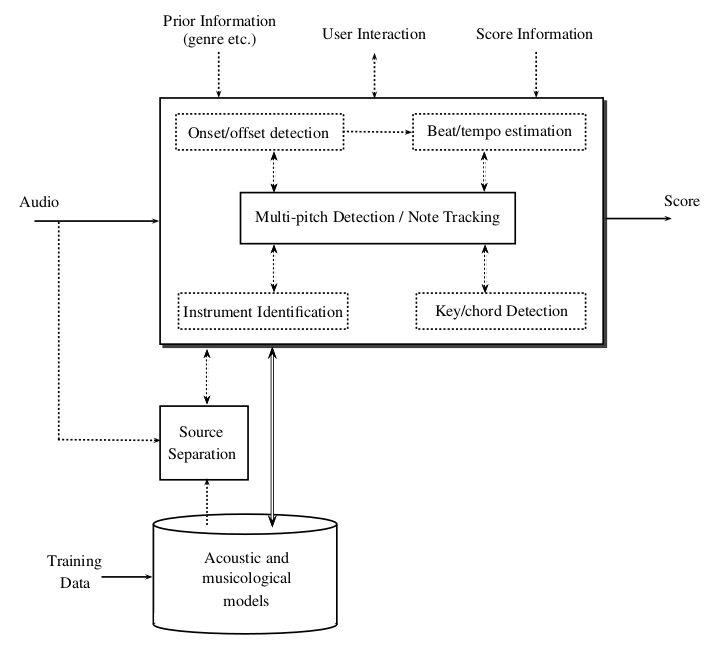
\includegraphics[height=60mm, width=60mm]{z_images/1_automatic_transcription/0_general_process.png}\\\\
\textit{Les sous-systèmes et algorithmes optionnels sont présentés à l'aide de lignes pointillées. Les doubles flèches mettent en évidence les connexions entre les systèmes qui incluent la fusion d'informations et une communication plus interactive entre les systèmes.}\\\\
Au cœur du système se trouvent les algorithmes de détection des multi-pitchs et de suivi des notes. Quatre sous-tâches de transcription liées à la détection des hauteurs multiples et au suivi des notes apparaissent comme des algorithmes facultatifs du système (cases en pointillé) qui peuvent être intégrés dans un système de transcription. Il s'agit de l'identification de l'instrument, de l'estimation de la tonalité et de l'accord, de la détection de l'apparition et du décalage, et de l'estimation du tempo et du rythme. La séparation des sources, un problème indépendant mais lié, pourrait être traitée par un système séparé qui pourrait informer et interagir avec le système de transcription en général, et plus spécifiquement avec le sous-système d'identification des instruments.
En option, des informations peuvent également être fournies de manière externe au système de transcription. Elles peuvent être données sous forme d'informations préalables (c'est-à-dire le genre, l'instrumentation, etc.), via l'interaction de l'utilisateur ou en fournissant des informations à partir d'une partition préexistante partiellement correcte ou incomplète. Enfin, les données de formation peuvent être utilisées pour apprendre des modèles acoustiques et musicologiques qui, par la suite, informent le système de transcription et interagissent avec lui. avec le système de transcription.
%\subsection{Exemple pour deux instruments}
%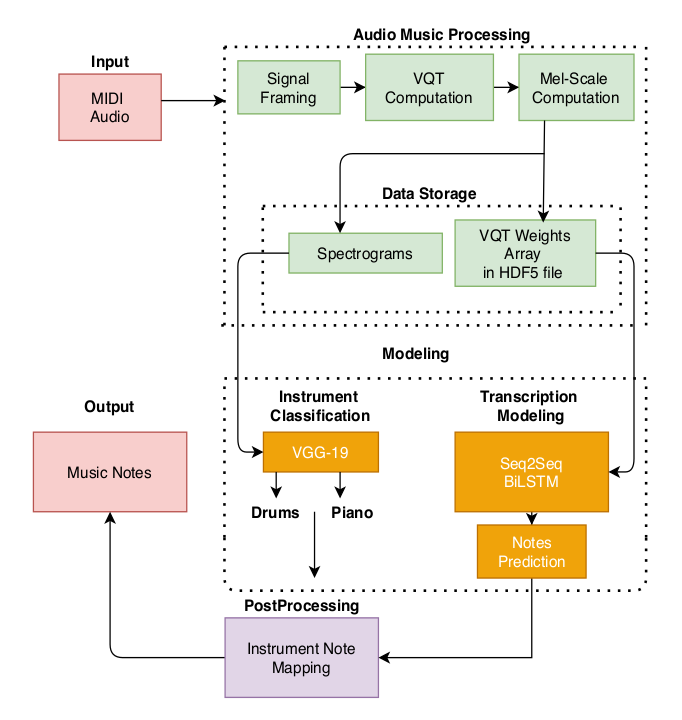
\includegraphics[height=60mm, width=60mm]{z_images/1_automatic_transcription/1_general_2instrus.png}\\
%\cite{article2}
%\subsection{Qparse}
%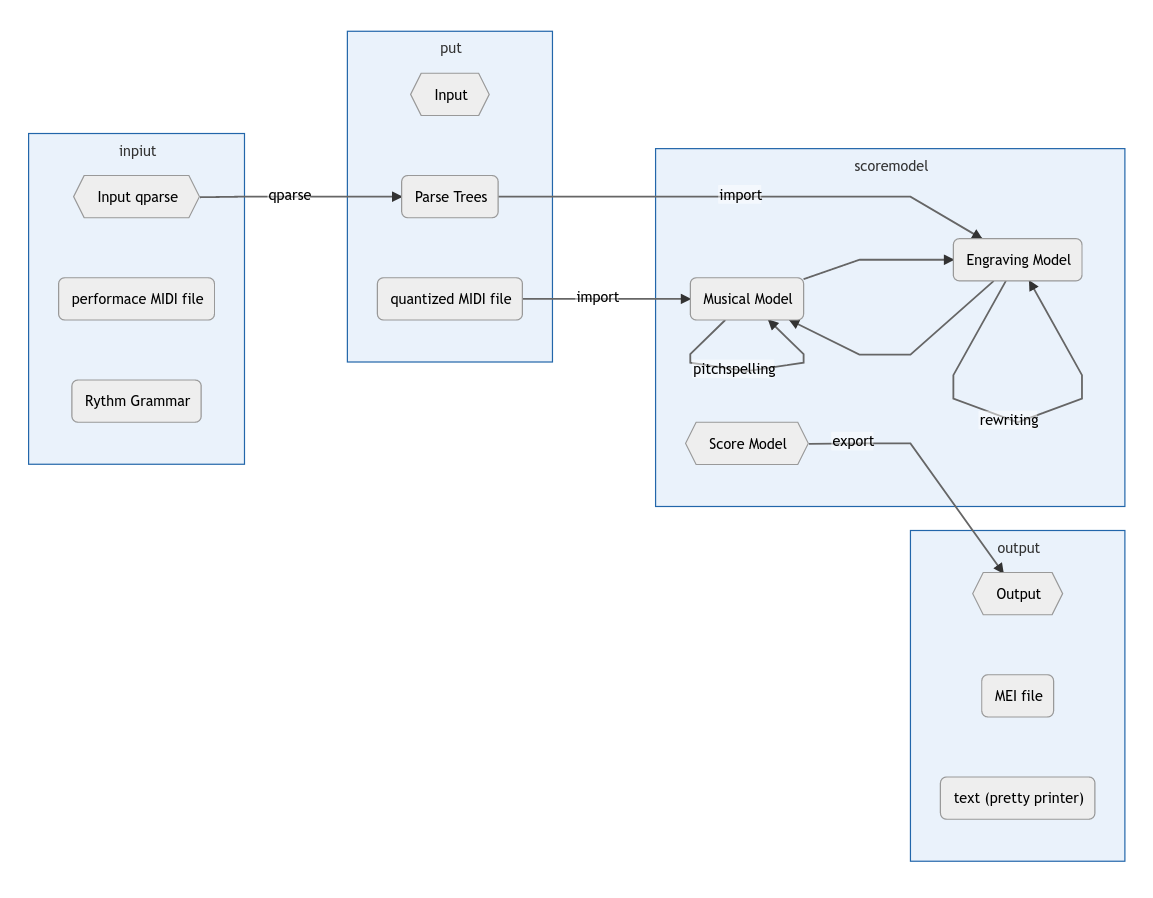
\includegraphics[height=60mm, width=60mm]{z_images/1_automatic_transcription/2_general_qparse.png}


\section{Transcription automatique de la batterie}
\subsection{Exemples de comparaisons de transcriptions pour la batterie}
\textit{drummer\_01/session3 — 10\_rock-folk\_90\_beat\_4-4}\\\\
Fichier midi vers partition avec musescore $\Rightarrow$ Transcription manuelle\\
\includegraphics[height=20mm, width=50mm]{z_images/transcriptions_manuelles/0_prise_en_main/0_tests_drummer_01__session3/musescore_0.png}\ \ \ \ 
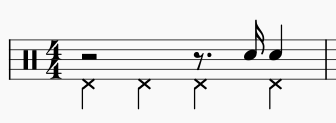
\includegraphics[height=20mm, width=55mm]{z_images/transcriptions_manuelles/0_prise_en_main/0_tests_drummer_01__session3/manuel_0.png}
\begin{itemize}
	\item Erreur d’indication de mesure ;
	\item Mauvaise transcription d’une noire.\\
\end{itemize}
La noire du 4ème temps se retrouve sur le premier temps de la mesure suivante et elle se transforme en un triolet de double croches dont seules les deux premières seraient jouées.\\\\
\textit{drummer\_01/session3 — 10\_rock-folk\_90\_beat\_4-4}\\\\
Fichier midi vers partition avec musescore $\Rightarrow$ Transcription manuelle\\
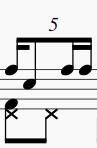
\includegraphics[height=20mm, width=15mm]{z_images/transcriptions_manuelles/0_prise_en_main/0_tests_drummer_01__session3/musescore_1.png}\ \ \ \ 
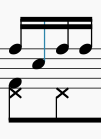
\includegraphics[height=20mm, width=15mm]{z_images/transcriptions_manuelles/0_prise_en_main/0_tests_drummer_01__session3/manuel_1.png}\\
\begin{itemize}
	\item Erreur de quantification : les doubles croches ont été interprétées en quintolet;\\
\end{itemize}
drummer\_01/session3 — 2\_jazz-swing\_185\_beat\_4-4
\\\\
Fichier midi vers partition avec musescore $\Rightarrow$ Transcription manuelle\\
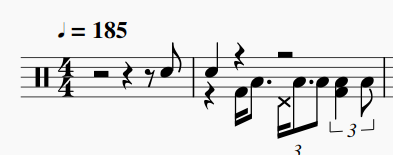
\includegraphics[height=25mm, width=60mm]{z_images/transcriptions_manuelles/0_prise_en_main/0_tests_drummer_01__session3/musescore_2.png}\ \ \ \ 
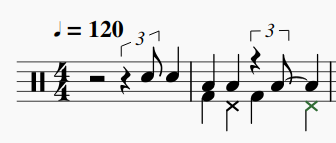
\includegraphics[height=25mm, width=55mm]{z_images/transcriptions_manuelles/0_prise_en_main/0_tests_drummer_01__session3/manuel_2.png}
\begin{itemize}
	\item L’indication de mesure est correcte mais tout a été décalé d’un temps car la première noire sur la caisse claire est jouée sur le 4ème temps et non sur le premier temps de la deuxième mesure comme l’indique la transcription de musescore.
	\item Les toms basses des 1er et 2ème temps de la mesure musescore auraient dû être sur les temps et non décalés d’une double croche vers la droite.\\
\end{itemize}
drummer\_01/session1 — 1\_funk\_80\_beat\_4-4\\\\
Fichier midi vers partition avec musescore $\Rightarrow$ Transcription manuelle\\
\includegraphics[height=25mm, width=40mm]{z_images/transcriptions_manuelles/0_prise_en_main/1_drummer_01__session1/musescore_0.png}\ \ \ \ 
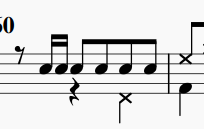
\includegraphics[height=25mm, width=40mm]{z_images/transcriptions_manuelles/0_prise_en_main/1_drummer_01__session1/Manuelle_0.png}
\begin{itemize}
	\item On dirait que lorsque certaines notes sont proches, elles se resserrent et suppriment celles qui aurait dû être sur le temps.\\
\end{itemize}
%drummer\_01/session1 — 1\_funk\_80\_beat\_4-4\\
%Fichier midi vers partition avec musescore :\\\\
%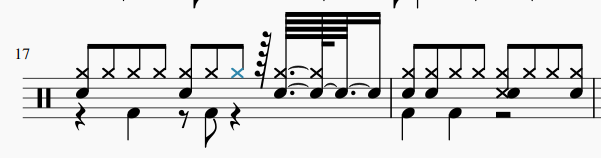
\includegraphics[height=25mm, width=80mm]{z_images/transcriptions_manuelles/0_prise_en_main/1_drummer_01__session1/MuseScore_1.png} \\\\
%Transcription manuelle :\\
%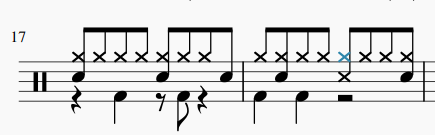
\includegraphics[height=20mm, width=65mm]{z_images/transcriptions_manuelles/0_prise_en_main/1_drummer_01__session1/Manuelle_1.png} \\
%\begin{itemize}
%	\item La caisse claire de la 2ème croche du 4ème temps de la 1ère mesure se transforme en une combinaison de quadruple/quintuple/double croches liées qui commence par un soupir et finit en débordant sur le premier temps de la mesure suivante. 
%\end{itemize}
\subsubsection{Exemple avec des flas}
%Des exemples de notation flas tom/caisse-claire existent dans des partitions récentes (rythmique binaire J.-F. Juskowiak).\\
%$\Rightarrow$ Ils faudra donc les prendre en compte dans les comparaisons de transcriptions.
Fichier midi vers partition avec musescore :\\
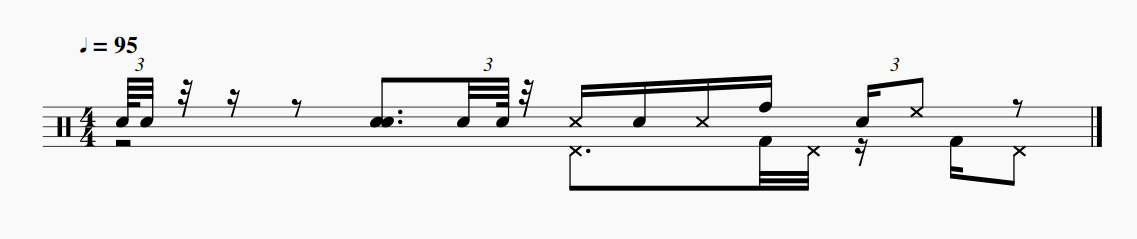
\includegraphics[height=30mm, width=120mm]{z_images/transcriptions_manuelles/1_transcriptions_flas/124_funk_95_fill_4-4_0.png}\\
Transcription manuelle :\\
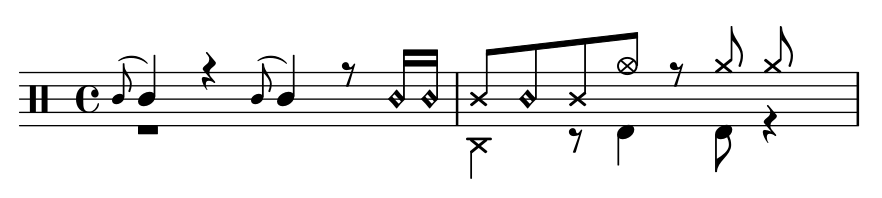
\includegraphics[height=20mm, width=90mm]{z_images/transcriptions_manuelles/1_transcriptions_flas/124_funk_95_fill_4-4_1_.png}\\
\subsection{Architecture Qparse}
En entrée : midi (séquence d’événements datés (piano roll) accompagné d’une grammaire pondérée)\\
$\Rightarrow$ parsing\\
$\Rightarrow$ global parsing tree\\
$\Rightarrow$ RI (Représentation Intermédiaire) arbres locaux par intruments\\
$\Rightarrow$ Sortie (xml, mei, lilypond,… )\\
Minimiser la distance entre le midi et la représentation en arbre.\\\\

\section{Conclusion}
Dans le cas, de l’ADT, l’architecture reste la même mais de nombreuse seront à affiner, notamment pour les questions de continuation ainsi que celle des ghost-notes et des accents.


%%%%%%%%%%%%%%%%%%%%%%%%%%%%%%%%%%%%%%%%%%%%%%%%%%%%%%
%% MÉTHODES
%%%%%%%%%%%%%%%%%%%%%%%%%%%%%%%%%%%%%%%%%%%%%%%%%%%%%%

\chapter{Méthodes}
\label{chap:methodes}
\minitoc

\textit{\\Méthodes (chapitre~\ref{chap:methodes})~: les méthodes
appliquées, avec le détail des expériences réalisées (différentes
configurations)~;}

\textit{\\Corpus (chapitre~\ref{chap:corpus})~: le corpus utilisé
	\emph{(caractéristiques, pré-traitements appliqués)}}

\section{Introduction}
Dans ce chapitre, nous expliquerons en détails les méthodes employées pour adapter à la batterie le processus décrit dans le chapitre précédent.
\newpage

\section{Généralités}
\subsection*{Chaîne de traitement}
\begin{itemize}
	\item Reconnaître un motif (système) sur une mesure de l’input (un fichier midi représentant des données audios)\\ $\Rightarrow$ Motif (système) reconnu : true ou false
	\item Si true : 
	\begin{itemize}
		\item Séparer les voix (\textit{Règles établis par le système})
		\item Simplifier l’écriture de chaque voix (\textit{Règles établis par le système})\\
	\end{itemize}
\end{itemize}
%Chaîne de traitement :\\
%if match(system\_parse\_tree(system + pitch), input\_midi\_parse\_tree)\\
%\tab then voice\_split ;\\
%\tab for voice in voice\_split:\\
%\tab \tab simplication voice

\subsection*{Références pour l’évaluation}
1 - Transcription manuelle à partir de fichier midi et/ou wav d’une partition contenant des systèmes. Écriture des systèmes contenues dans la partition (arbres, séparation des voix, réécriture)

\section{Représentations, systèmes et réécriture}

\subsection{La notation de la batterie}
\subsubsection{La hauteur des notes et les têtes de notes}
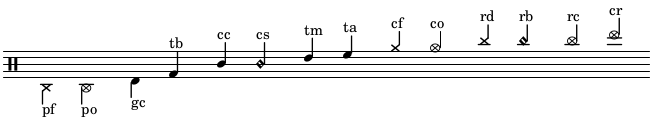
\includegraphics[height=30mm, width=155mm]{z_images/1_description_notation/notes.png}
partition 1
\subsubsection{Les nuances}
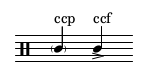
\includegraphics[height=20mm, width=35mm]{z_images/1_description_notation/nuances.png}\\
partition 2\\\\
Bien expliquer les accents, remplacer p et f par g et a\\
$\Rightarrow$ nuance VS articulation\\
\subsubsection{La séparation des voix}
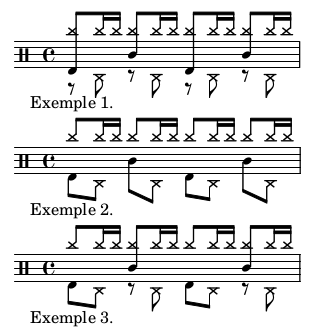
\includegraphics[height=65mm, width=60mm]{z_images/1_description_notation/separation/0_exemples_separation.png}\\
partition 3
\subsection{La notation midi de la batterie}
\subsubsection{Représentation symbolique (MIDI)}
………\\
\subsubsection{Les pitchs et la vélocité}
\begin{table}[h]
	\centering
	\begin{tabular}{|c|c|c|} \hline
		Codes & Instruments & Pitchs \\ \hline
		cf & charley-main-fermé & 22, 42 \\
		co & charley-main-ouvert & 26 \\
		pf & charley-pied-fermé & 44 \\
		rd & ride & 51 \\
		rb & ride-cloche (bell) & 53 \\
		rc & ride-crash & 59 \\
		cr & crash & 55 \\
		cc & caisse-claire & 38, 40 \\
		cs & cross-stick & 37 \\
		ta & tom-alto & 48, 50 \\
		tm & tom-medium & 45, 47 \\
		tb & tom-basse & 43, 58 \\
		gc & grosse-caisse & 36 \\ \hline
	\end{tabular}
	\caption{Pitchs et instruments}
	%	\label{tab:exemple}
\end{table}
\begin{table}[h]
	\centering
	\begin{tabular}{|c|c|c|c|} \hline
		Codes & Instruments & Pitchs & Vélocité \\ \hline
		cop & charley-main-ouvert & 46 & ? \\ \hline
	\end{tabular}
	\caption{Vélocité et nuances}
\end{table}
Pas de charley pied ouvert…
Nous ne prendrons en compte la vélocité que pour la cc, les toms et les cymbales jouées aux mains. Les nuances de grosse caisse et charley aux pieds sont le plus souvent insignifiantes, elles ne sont marquées sur le figure qu’à titre indicatif.\\\\
Si la vélocité est en dessous de 40, il s’agit de ghost-notes : la tête de note devra être entouré de parenthèses et le suffixe \textit{p (piano)} devra être ajouté au codes de l’instrument. (Voir ccp ci-dessus.)\\\\
Si la vélocité est au dessus de 90, il s’agit de notes accentuées : le symbole « > » et le suffixe \textit{f (forte)} devra être ajouté au codes de l’instrument. (Voir ccf ci-dessus.)\\\\
Lorsque la vélocité va de 40 à 89, on considèrera le volume comme normal et aucun symbole supplémentaire ne sera ajouté à la note.\\\\
L’instrument qui sera difficile à placer sera la caisse claire car elle ne sera pas toujours affiliée aux mêmes instruments.
\subsubsection{Les dilemmes}
Le charley de pitch 46 est considéré comme le charley ouvert joué à la main sur le haut de la cymbale mais souvent, ça correspond au geste « tranche-olive » de la baguette lorsque le batteur accentue avec la tranche et joue moins fort avec l’olive sur le plat de la cymbale. Je vais dans un premier temps considérer le pitch comme \textbf{charley-main-ouvert-piano} (ghost-note)
\newpage
\subsubsection{Représentations en arbres}
Voici une représentation de la \textit{partition 3} en arbre de rythme avec les codes de chaque instrument :\\\\
\Tree[ [ [rd\\gc ][ [rd\\pf ][rd ]]]
[ [rd\\cc ][ [rd\\pf ][rd ]]]
[ [rd\\gc ][ [rd\\pf ][rd ]]]
[ [rd\\cc ][ [rd\\pf ][rd ]]] ]\\\\\\
Ci-dessous, le même arbre dont les codes des instruments sont remplacés par leurs données midi respectives :\\\\
\Tree[ [ [51\\36 ][ [51\\44 ][51 ]]]
[ [51\\38 ][ [51\\44 ][51 ]]]
[ [51\\36 ][ [51\\44 ][51 ]]]
[ [51\\38 ][ [51\\44 ][51 ]]] ]\\\\\\
Cet arbre représente un rythme unique dont les possiblités de notation sur une partition sont théoriquement multiples.(Voir \textit{partition 3}).\newpage
\subsection{Les systèmes}
\subsubsection{Définition}

Un système est la combinaison d’un ou plusieurs éléments qui jouent un rythme en boucle (motif) et d’un autre élément qui joue un texte rythmique variable mais respectant les règles propre au système (gamme).\\

Système = motif + gamme/texte\\
motif = rythmes coordonnés joués avec 2 ou 3 membres en boucle (reparti sur 1 ou 2 voix)\\
gamme/texte = rythme irrégulier joué avec un seul membre sur le motif (Réparti sur 1 voix). La gamme d’un système considère l’ensemble des combinaisons que le batteur pourrait rencontrer en interprétant un texte rythmique à l’aide du système.\\

Nous partirons de propositions génériques de systèmes (environs trois systèmes dans différents styles de batterie) que nous tenterons de détecter dans le jeu de données groove.\\

Quatre systèmes standards :
\begin{itemize}
	\item binaire
	\item ternaire (shuffle, afro, rock)
	\item jazz
	\item afro-cubain\\
\end{itemize}

Nous travaillerons aussi sur la détection de répétitions sur plusieurs mesures afin de pouvoir corriger des erreurs sur une des mesures qui aurait dû être identique aux autres mais qui présente des différences.

\subsubsection{Utilité}
\begin{itemize}
	\item Séparation des voix
	\item Définir une métrique
	\item Conditionner des règles spécifiques de réécriture
\end{itemize}

Créer un ensemble de systèmes :
\begin{itemize}
	\item 4/4 binaire FAIT
	\item jazz vs ternaire(12/8) EN COURS…
	\item afro-cubain
	\item Tout transcrire avec lilypond et en arbres d’analyse syntaxique.
	\item Créer les arbres de voix séparées.
	\item Écrire les règles de réécriture.
	\item Créer les arbres de voix séparées simplifiés (rewriting).\\	
\end{itemize}

Pour la \textbf{séparation des voix} et la \textbf{définition des métriques}, nous nous intéresserons principalement à la partie \textit{motif} des systèmes qui seront présentés. La partie \textit{texte} nous intéressera plus pour les \textbf{combinaisons de réécritures}.
\newpage
\subsubsection{Pour la séparation des voix}
\textbf{Motif 4-4 binaire}\\\\
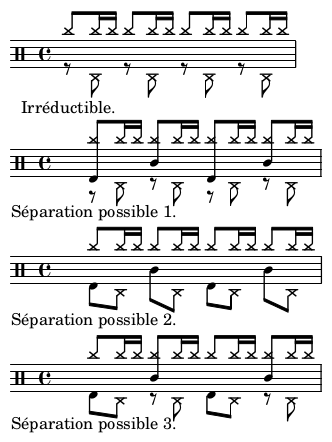
\includegraphics[height=60mm, width=40mm]{z_images/1_description_notation/separation/1_separation_4-4_binaire.png}\\\\
Ici, le système est construit sur un modèle rock en 4/4 : after-beat sur les 2 et 4 avec un choix de répartition des cymbales type fast-jazz. Le système est constitué par défaut du motif ride/ch-pf/cc et d’un texte joué à la grosse-caisse. La troisième séparation proposée est privilégiée car elle répartit selon 2 voix, une voix pour les mains (ride + cc) et une voix pour les pieds (ch-pf + gc). Ce choix paraît plus équilibré car deux instruments sont utilisés par voix et plus logique pour le lecteur puisque les mains sont en haut et les pieds en bas.\\
%D’autres choix d’écriture auraient été possibles :
%\begin{itemize}
%	\item Toutes les hampes en haut ;
%	\item Combinaison motif 1 et 2 en donnant 2 directions aux hampes de la cc).\\
%\end{itemize}

\textbf{Motif 4-4 jazz}\\\\
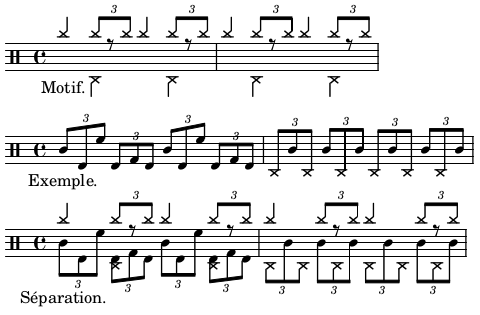
\includegraphics[height=45mm, width=60mm]{z_images/1_description_notation/separation/2_separation_4-4_jazz.png}\\\\
Dans la plupart des méthodes, le charley n’est pas écrit car considéré comme évident en jazz traditionnel. Ce qui facilite grandement l’écriture : la ride et les crash sur la voix du haut et le reste sur la voix du bas. Ici, le partie prit et de tout écrire. Dans l’exemple ci-dessus, les mesures 1 et 2 combinées avec le \textit{motif} de la première ligne, sont des cas typiques de la batterie jazz. Tout mettre sur la voix haute serait surchargé. De plus, la grosse caisse entre très souvent dans le flot des combinaisons de toms et de caisse claire et son écriture séparée serait inutilement compliquée et peu intuitive pour le lecteur. Le choix de séparation sera donc de laisser les cymbales en haut et toms, caisse-claire, grosse-caisse et pédale de charley en bas.
\newpage

\textbf{Système 4-4 afro-cubain}\\\\
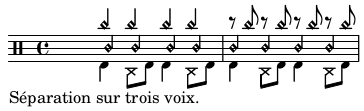
\includegraphics[height=25mm, width=80mm]{z_images/1_description_notation/separation/3_separation_afro-cubain.png}\\\\

\subsubsection{Pour la reconnaissance de la métrique}
\textit{\textbf{12/8 vs 4/4 ternaire}}\\\\
\textbf{Motif 12/8}\\\\
%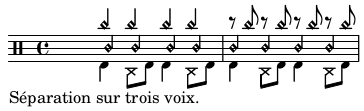
\includegraphics[height=30mm, width=100mm]{z_images/1_description_notation/separation/separation_2.png}\\\\

\subsubsection{Pour les règles de réécriture}
Les textes qui accompagnent les motifs étayent toutes les combinaisons d’un systèmes. 
\newpage

%\subsubsection{Construction des systèmes pour les expérimentations}
















\subsubsection*{La réécriture des évènements MIDI pour la batterie}
Basé sur \cite{jacquemard:hal-01134096} et sur \cite{jacquemard:hal-01403982}\\
Pour la plupart des instruments mélodiques, la liaison et le point sont les deux seules possibilités en cas d’équivalence rythmique pour des notes dont la durée de l’une à l’autre est ininterrompue. Mais puisque les durées des notes n’ont pas d’importance en batterie, l’usage des silences pour combler la distance rythmique entre deux notes devient possible.\\Les cymbales-crash et les ouvertures de charley constituent le seul cas qui exclut cette option. Le charley car ses ouvertures/fermetures sont presque toujours quantifiées et les cymbales-crash car elles peuvent être arrêtées à la main de manière quantifié aussi mais ce cas est très rare, nous allons donc nous concentrer sur les ouvertures de charley et considérer les crashs comme des événements sans durée.\\\\
Les fermetures du charley sont notées soit par un silence (correspondant à une fermeture de la pédale), soit par un écrasement de l’ouverture par un autre coup de charley fermé, au pied ou à la main.\\\\
\textbf{Exemples} :\\
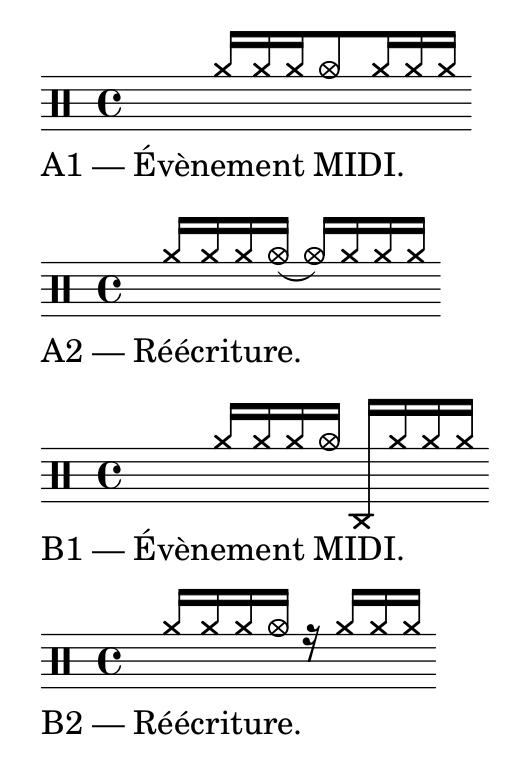
\includegraphics[height=80mm, width=60mm]{z_images/reecriture/exemples_charley_1.png}\\\\

\textbf{Exemples à écrire en arbre :}\\
\begin{itemize}
	\item 
	SI (pas pf) ET (note sur un temps suivie de note en l’air) :\\
	$\Rightarrow$ (Temps1 : Note pertinente) + (Temps2 : Silence pertinent + Note pertinente.)\\
	\item
	Si (po ou co) déborde sur le temps suivant :\\
	$\Rightarrow$ Liaison car marchera dans tous les cas même la où le point ne marchera pas (voir A2).\\
	\item
	Une blanche sera écrite noir + soupir.\\\\
\end{itemize}
\subsubsection{Les régles de réécriture}
~~\\
\Tree[.$\frac{2}{8}$ [.x ][.tie ]]\Tree[.2/8 [.x ]]\\\\\\
\Tree[.1/4 [.x ][.tie ]]\Tree[.1/4 [.x ][.r ]]\\\\\\

\section{Évaluation}
\subsubsection{Comparaison d’arbres}

Trouver un moyen de comparer l’arbre obtenu automatiquement de l’arbre de la transcription manuelle.

\section{Conclusion}
Conclusion de ce chapitre.


%%%%%%%%%%%%%%%%%%%%%%%%%%%%%%%%%%%%%%%%%%%%%%%%%%%%%%%%%%%%%%%%
%% Deuxième partie

\part{Expérimentations}

%%%%%%%%%%%%%%%%%%%%%%%%%%%%%%%%%%%%%%%%%%%%%%%%%%%%%%
%% CORPUS
%%%%%%%%%%%%%%%%%%%%%%%%%%%%%%%%%%%%%%%%%%%%%%%%%%%%%%


\chapter{Corpus}
\label{chap:corpus}
\minitoc

\section{Introduction}
Dans ce chapitre, nous présenterons le corpus, les expérimentations et les différents choix effectués pour les tests.

\section{Le corpus}
\textbf{groove MIDI dataset}\\
	\url{https://magenta.tensorflow.org/datasets/groove}\\\\
	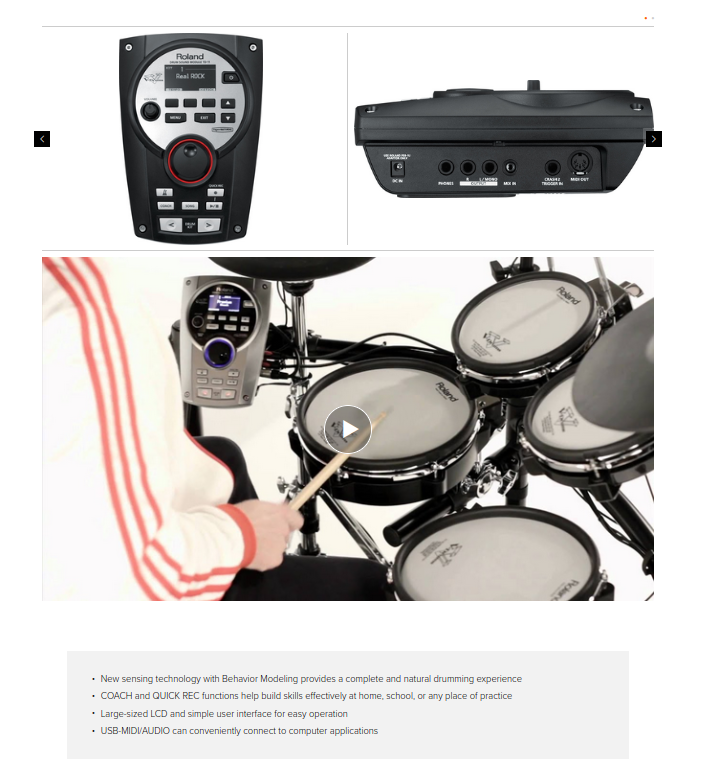
\includegraphics[height=60mm, width=60mm]{z_images/2_groove/roland_TD11.png}\\
	Des batteurs pro ont été engagés pour jouer sur un roland td-11\\\\
	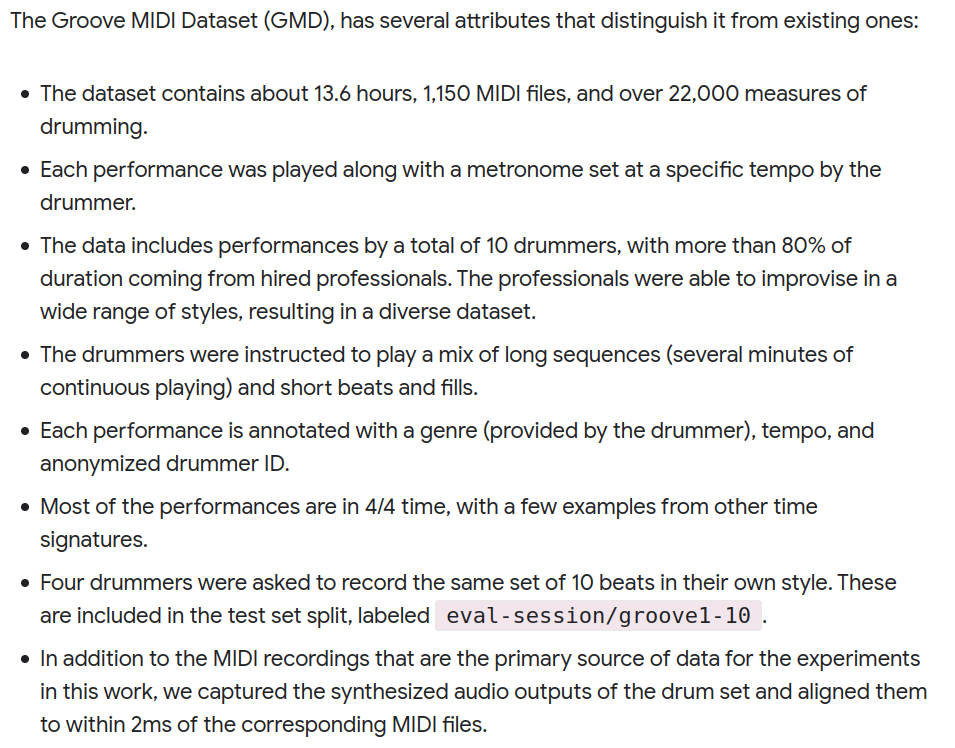
\includegraphics[height=80mm, width=110mm]{z_images/2_groove/dataset_how.png}\newpage{}
	\textbf{Les métadatas :}\\\\
	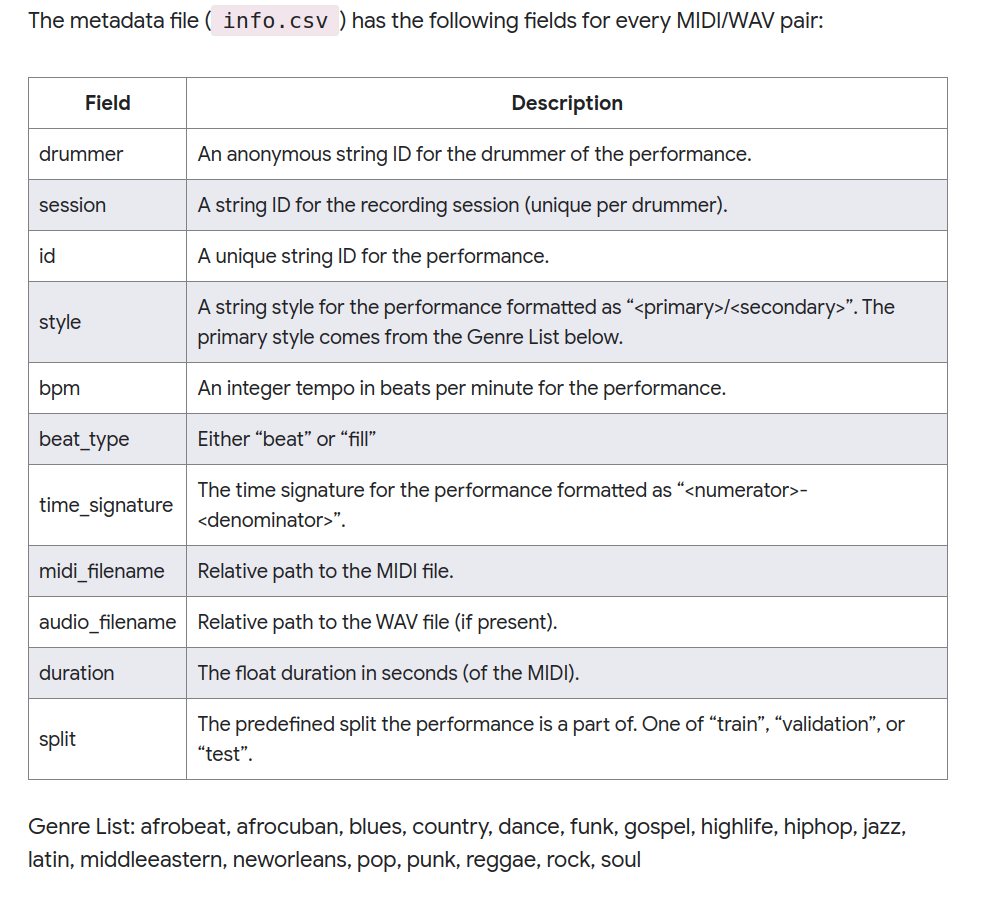
\includegraphics[height=85mm, 
	width=100mm]{z_images/2_groove/csv_metadata_struct.png}\\
	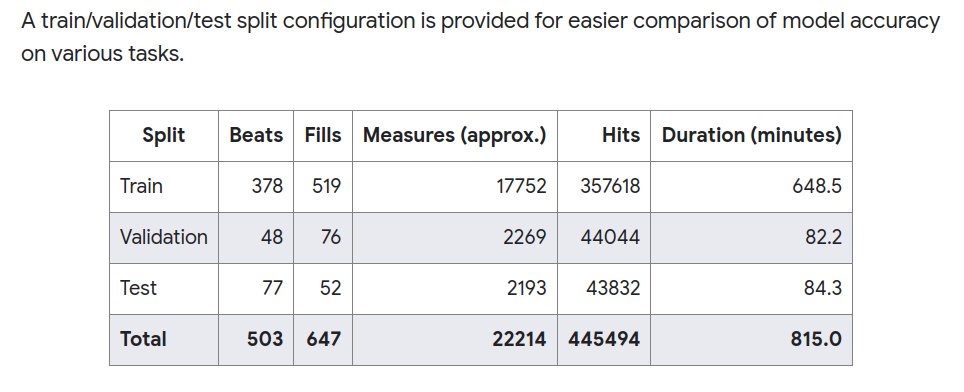
\includegraphics[height=50mm, width=120mm]{z_images/2_groove/train_validation_test.png}\\
	Détails (entre autres tensorflow avec le dataset) à :
	\url{https://magenta.tensorflow.org/datasets/groove#license}\\
	écouter le dataset groove
	\newpage
\section{Choix pour les tests}
\subsection{Expérience 1 - 4/4 binaire}
\subsubsection{Partition de référence pour l’ouput}
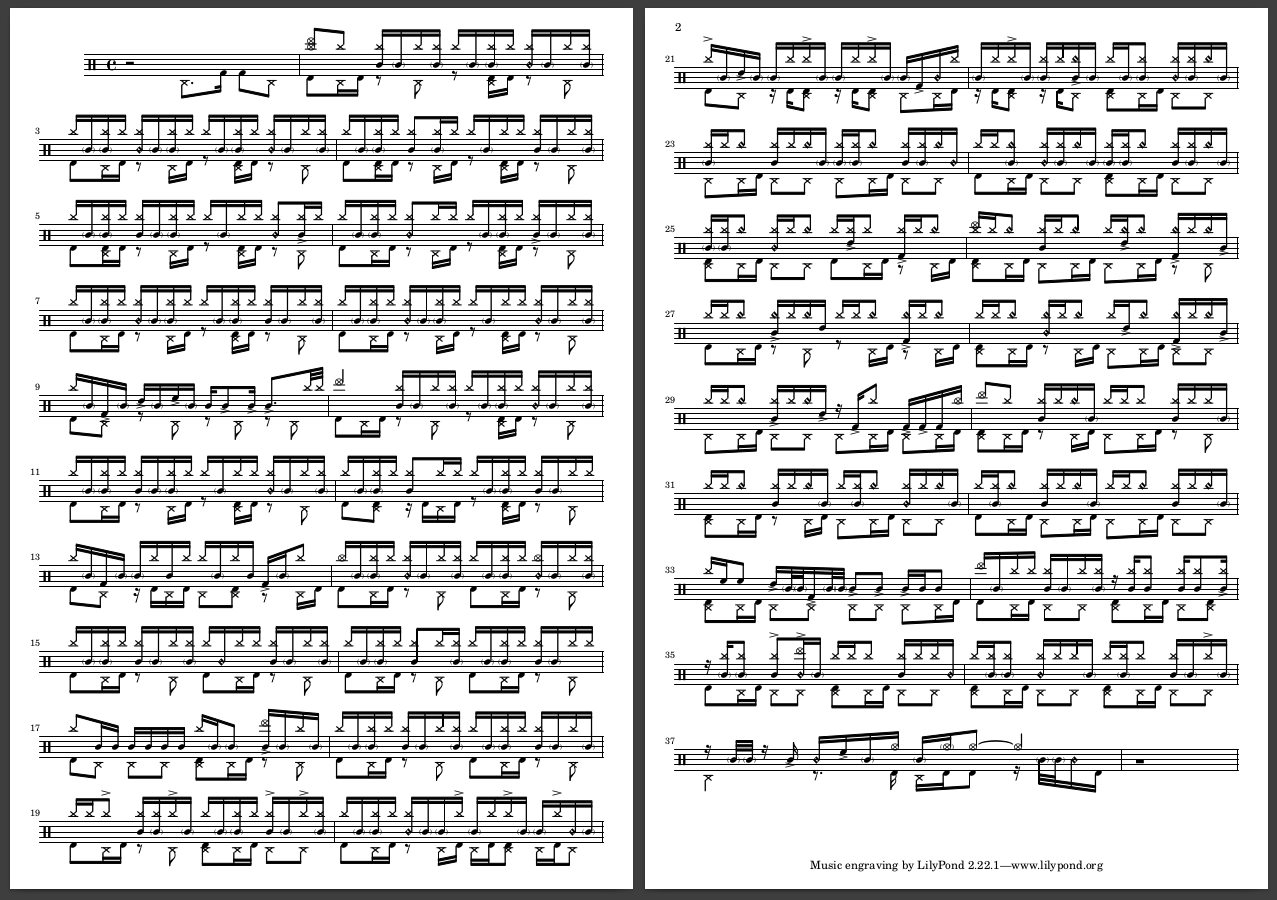
\includegraphics[height=120mm, width=160mm]{z_images/3_experimentations/experience_1/partition.png}
\subsubsection{Systèmes recherchés}
Textes :\\\\
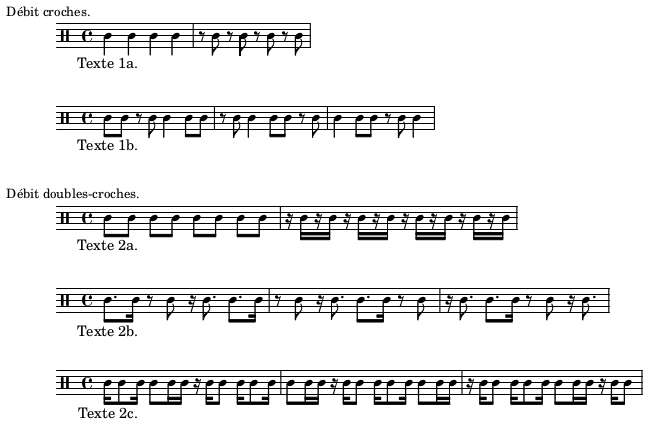
\includegraphics[height=70mm, width=95mm]{z_images/1_description_notation/systemes/0_textes_4-4_binaires.png}\\
Motifs :\\\\
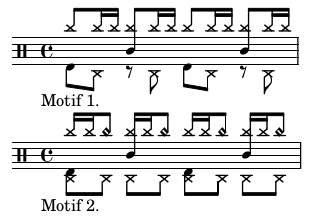
\includegraphics[height=30mm, width=40mm]{z_images/1_description_notation/systemes/1_motifs_4-4_binaires.png}\\\\
Systèmes résultants :\\\\
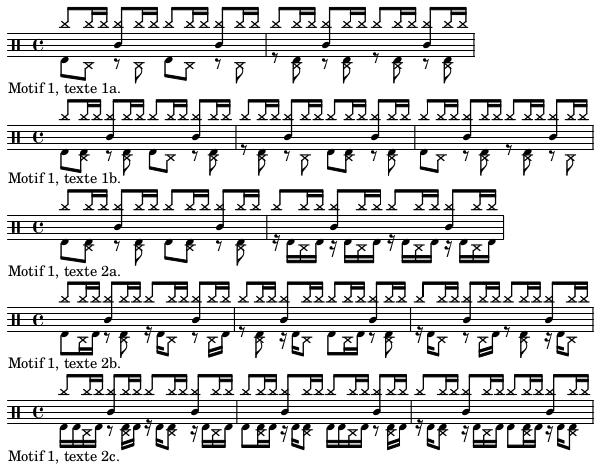
\includegraphics[height=75mm, width=85mm]{z_images/3_experimentations/experience_1/systeme_recherche_1.png}
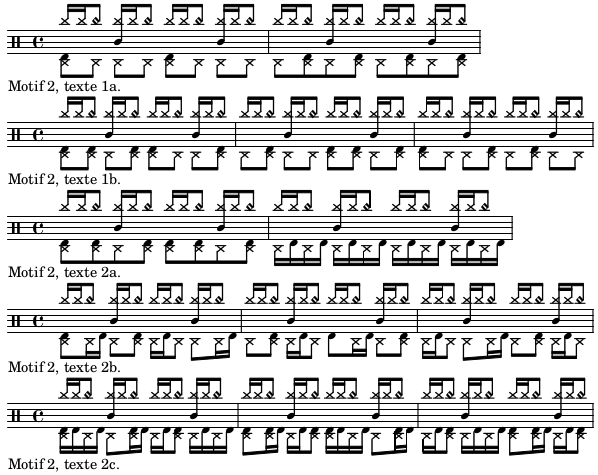
\includegraphics[height=75mm, width=85mm]{z_images/3_experimentations/experience_1/systeme_recherche_2.png}


\subsubsection{Représentation des systèmes en arbres de rythmes}

\resizebox{500pt}{!} {
	\Tree[.Motif\ 1\ +\ Texte\ 1a
	[.Mesure\ 1
	[.Temps\ 1 [rd\\bd ][ [rd\\pf ][rd ]]]
	[.Temps\ 2 [rd\\cc ][ [rd\\pf ][rd ]]]
	[.Temps\ 3 [rd\\bd ][ [rd\\pf ][rd ]]]
	[.Temps\ 4 [rd\\cc ][ [rd\\pf ][rd ]]] ]
	[.Mesure\ 2
	[.Temps\ 1 [rd ][ [rd\\bd\\pf ][rd ]]]
	[.Temps\ 2 [rd\\cc ][ [rd\\bd\\pf ][rd ]]]
	[.Temps\ 3 [rd ][ [rd\\bd\\pf ][rd ]]]
	[.Temps\ 4 [rd\\cc ][ [rd\\bd\\pf ][rd ]]] ]]}\\

\resizebox{500pt}{!} {
	\Tree[.Motif\ 1\ +\ Texte\ 1b
	[.Mesure\ 1
	[.Temps\ 1 [rd\\bd ][ [rd\\bd\\pf ][rd ]]]
	[.Temps\ 2 [rd\\cc ][ [rd\\bd\\pf ][rd ]]]
	[.Temps\ 3 [rd\\bd ][ [rd\\pf ][rd ]]]
	[.Temps\ 4 [rd\\cc ][ [rd\\bd\\pf ][rd ]]] ]
	[.Mesure\ 2
	[.Temps\ 1 [rd ][ [rd\\bd\\pf ][rd ]]]
	[.Temps\ 2 [rd\\cc ][ [rd\\pf ][rd ]]]
	[.Temps\ 3 [rd\\bd ][ [rd\\bd\\pf ][rd ]]]
	[.Temps\ 4 [rd\\cc ][ [rd\\bd\\pf ][rd ]]] ]
	[.Mesure\ 3
	[.Temps\ 1 [rd\\bd ][ [rd\\pf ][rd ]]]
	[.Temps\ 2 [rd\\cc ][ [rd\\bd\\pf ][rd ]]]
	[.Temps\ 3 [rd ][ [rd\\bd\\pf ][rd ]]]
	[.Temps\ 4 [rd\\cc ][ [rd\\pf ][rd ]]] ]]}\\

\resizebox{500pt}{!} {
	\Tree[.Motif\ 1\ +\ Texte\ 2a
	[.Mesure\ 1
	[.Temps\ 1 [rd\\bd ][ [rd\\bd\\pf ][rd ]]]
	[.Temps\ 2 [rd\\cc ][ [rd\\bd\\pf ][rd ]]]
	[.Temps\ 3 [rd\\bd ][ [rd\\bd\\pf ][rd ]]]
	[.Temps\ 4 [rd\\cc ][ [rd\\bd\\pf ][rd ]]] ]
	[.Mesure\ 2
	[.Temps\ 1 [rd ][bd ][rd\\pf ][rd\\bd ]]
	[.Temps\ 2 [rd\\cc ][bd ][rd\\pf ][rd\\bd ]]
	[.Temps\ 3 [rd ][bd ][rd\\pf ][rd\\bd ]]
	[.Temps\ 4 [rd\\cc ][bd ][rd\\pf ][rd\\bd ]] ]]}\\

\resizebox{500pt}{!} {
	\Tree[.Motif\ 1\ +\ Texte\ 2b
	[.Mesure\ 1
	[.Temps\ 1 [rd\\bd ][ [rd\\pf ][rd\\bd ]]]
	[.Temps\ 2 [rd\\cc ][ [rd\\bd\\pf ][rd ]]]
	[.Temps\ 3 [rd ][bd ][rd\\pf ][rd ]]
	[.Temps\ 4 [rd\\cc ][ [rd\\pf ][rd\\bd ]]] ]
	[.Mesure\ 2
	[.Temps\ 1 [rd\\ ][ [rd\\bd\\pf ][rd ]]]
	[.Temps\ 2 [rd\\cc ][bd ][rd\\pf ][rd ]]
	[.Temps\ 3 [rd\\bd ][ [rd\\pf ][rd\\bd ]]]
	[.Temps\ 4 [rd\\cc ][ [rd\\bd\\pf ][rd ]]] ]
	[.Mesure\ 3
	[.Temps\ 1 [rd ][bd ][rd\\pf ][rd ]]
	[.Temps\ 2 [rd\\cc ][ [rd\\pf ][rd\\bd ]]]
	[.Temps\ 3 [rd ][ [rd\\bd\\pf ][rd ]]]
	[.Temps\ 4 [rd\\cc ][bd ][rd\\pf ][rd ]]] ] }\\

\resizebox{500pt}{!} {
	\Tree[.Motif\ 1\ +\ Texte\ 2c
	[.Mesure\ 1
	[.Temps\ 1 [rd\\bd ][bd ][rd\\pf ][rd\\bd ]]
	[.Temps\ 2 [rd\\cc ][ [rd\\bd\\pf ][rd\\bd ]]]
	[.Temps\ 3 [rd ][bd ][rd\\bd\\pf ][rd ]]
	[.Temps\ 4 [rd\\cc ][bd ][rd\\pf ][rd\\bd ]] ]
	[.Mesure\ 2
	[.Temps\ 1 [rd\\bd ][ [rd\\bd\\pf ][rd\\bd ]]]
	[.Temps\ 2 [rd\\cc ][bd ][rd\\bd\\pf ][rd ]]
	[.Temps\ 3 [rd\\bd ][bd ][rd\\pf ][rd\\bd ]]
	[.Temps\ 4 [rd\\cc ][ [rd\\bd\\pf ][rd\\bd ]]] ]
	[.Mesure\ 3
	[.Temps\ 1 [rd ][bd ][rd\\bd\\pf ][rd ]]
	[.Temps\ 2 [rd\\cc ][bd ][rd\\pf ][rd\\bd ]]
	[.Temps\ 3 [rd\\bd ][ [rd\\bd\\pf ][rd\\bd ]]]
	[.Temps\ 4 [rd\\cc ][bd ][rd\\bd\\pf ][rd ]]] ] }\\\\

\subsubsection{Séparation des voix}
Motif\ 1\ +\ Texte\ 1a\\\\
\textit{Voix haute}\\
\resizebox{500pt}{!} {
	\Tree[.Motif\ 1\ +\ Texte\ 1a
	[.Mesure\ 1
	[.Temps\ 1 [rd ][ [rd ][rd ]]]
	[.Temps\ 2 [rd\\cc ][ [rd ][rd ]]]
	[.Temps\ 3 [rd ][ [rd ][rd ]]]
	[.Temps\ 4 [rd\\cc ][ [rd ][rd ]]] ]
	[.Mesure\ 2
	[.Temps\ 1 [rd ][ [rd ][rd ]]]
	[.Temps\ 2 [rd\\cc ][ [rd ][rd ]]]
	[.Temps\ 3 [rd ][ [rd ][rd ]]]
	[.Temps\ 4 [rd\\cc ][ [rd ][rd ]]] ]]}\\

\textit{Voix basse}\\
\resizebox{500pt}{!} {
	\Tree[.Motif\ 1\ +\ Texte\ 1a
	[.Mesure\ 1
	[.Temps\ 1 [bd ][ [pf ][t ]]]
	[.Temps\ 2 [t ][ [pf ][t ]]]
	[.Temps\ 3 [bd ][ [pf ][t ]]]
	[.Temps\ 4 [t ][ [pf ][t ]]] ]
	[.Mesure\ 2
	[.Temps\ 1 [t ][ [bd\\pf ][t ]]]
	[.Temps\ 2 [t ][ [bd\\pf ][t ]]]
	[.Temps\ 3 [t ][ [bd\\pf ][t ]]]
	[.Temps\ 4 [t ][ [bd\\pf ][t ]]] ]]}\\

Motif\ 1\ +\ Texte\ 1b\\\\
\textit{Voix haute}\\
\resizebox{500pt}{!} {
	\Tree[.Motif\ 1\ +\ Texte\ 1b
	[.Mesure\ 1
	[.Temps\ 1 [rd ][ [rd ][rd ]]]
	[.Temps\ 2 [rd\\cc ][ [rd ][rd ]]]
	[.Temps\ 3 [rd ][ [rd ][rd ]]]
	[.Temps\ 4 [rd\\cc ][ [rd ][rd ]]] ]
	[.Mesure\ 2
	[.Temps\ 1 [rd ][ [rd ][rd ]]]
	[.Temps\ 2 [rd\\cc ][ [rd ][rd ]]]
	[.Temps\ 3 [rd ][ [rd ][rd ]]]
	[.Temps\ 4 [rd\\cc ][ [rd ][rd ]]] ]
	[.Mesure\ 3
	[.Temps\ 1 [rd ][ [rd ][rd ]]]
	[.Temps\ 2 [rd\\cc ][ [rd ][rd ]]]
	[.Temps\ 3 [rd ][ [rd ][rd ]]]
	[.Temps\ 4 [rd\\cc ][ [rd ][rd ]]] ]]}\\

\textit{Voix basse}\\
\resizebox{500pt}{!} {
	\Tree[.Motif\ 1\ +\ Texte\ 1b
	[.Mesure\ 1
	[.Temps\ 1 [bd ][ [bd\\pf ][t ]]]
	[.Temps\ 2 [t ][ [bd\\pf ][t ]]]
	[.Temps\ 3 [bd ][ [pf ][t ]]]
	[.Temps\ 4 [t ][ [bd\\pf ][t ]]] ]
	[.Mesure\ 2
	[.Temps\ 1 [t ][ [bd\\pf ][t ]]]
	[.Temps\ 2 [t ][ [pf ][t ]]]
	[.Temps\ 3 [bd ][ [bd\\pf ][t ]]]
	[.Temps\ 4 [t ][ [bd\\pf ][t ]]] ]
	[.Mesure\ 3
	[.Temps\ 1 [bd ][ [pf ][t ]]]
	[.Temps\ 2 [t ][ [bd\\pf ][t ]]]
	[.Temps\ 3 [t ][ [bd\\pf ][t ]]]
	[.Temps\ 4 [t ][ [pf ][t ]]] ]]}\\

Motif\ 1\ +\ Texte\ 2a\\\\
\textit{Voix haute}\\
\resizebox{500pt}{!} {
	\Tree[.Motif\ 1\ +\ Texte\ 2a
	[.Mesure\ 1
	[.Temps\ 1 [rd ][ [rd ][rd ]]]
	[.Temps\ 2 [rd\\cc ][ [rd ][rd ]]]
	[.Temps\ 3 [rd ][ [rd ][rd ]]]
	[.Temps\ 4 [rd\\cc ][ [rd ][rd ]]] ]
	[.Mesure\ 2
	[.Temps\ 1 [rd ][t ][rd ][rd ]]
	[.Temps\ 2 [rd\\cc ][t ][rd ][rd ]]
	[.Temps\ 3 [rd ][t ][rd ][rd ]]
	[.Temps\ 4 [rd\\cc ][t ][rd ][rd ]] ]]}\\

\textit{Voix basse}\\
\resizebox{500pt}{!} {
	\Tree[.Motif\ 1\ +\ Texte\ 2a
	[.Mesure\ 1
	[.Temps\ 1 [bd ][ [bd\\pf ][t ]]]
	[.Temps\ 2 [t ][ [bd\\pf ][t ]]]
	[.Temps\ 3 [bd ][ [bd\\pf ][t ]]]
	[.Temps\ 4 [t ][ [bd\\pf ][t ]]] ]
	[.Mesure\ 2
	[.Temps\ 1 [t ][bd ][pf ][bd ]]
	[.Temps\ 2 [t ][bd ][pf ][bd ]]
	[.Temps\ 3 [t ][bd ][pf ][bd ]]
	[.Temps\ 4 [t ][bd ][pf ][bd ]] ]]}\\

Motif\ 1\ +\ Texte\ 2b\\\\
\textit{Voix haute}\\
\resizebox{500pt}{!} {
	\Tree[.Motif\ 1\ +\ Texte\ 2b
	[.Mesure\ 1
	[.Temps\ 1 [rd ][ [rd ][rd ]]]
	[.Temps\ 2 [rd\\cc ][ [rd ][rd ]]]
	[.Temps\ 3 [rd ][t ][rd ][rd ]]
	[.Temps\ 4 [rd\\cc ][ [rd ][rd ]]] ]
	[.Mesure\ 2
	[.Temps\ 1 [rd\\ ][ [rd ][rd ]]]
	[.Temps\ 2 [rd\\cc ][t ][rd ][rd ]]
	[.Temps\ 3 [rd ][ [rd ][rd ]]]
	[.Temps\ 4 [rd\\cc ][ [rd ][rd ]]] ]
	[.Mesure\ 3
	[.Temps\ 1 [rd ][t ][rd ][rd ]]
	[.Temps\ 2 [rd\\cc ][ [rd ][rd ]]]
	[.Temps\ 3 [rd ][ [rd ][rd ]]]
	[.Temps\ 4 [rd\\cc ][t ][rd ][rd ]]] ] }\\

\textit{Voix basse}\\
\resizebox{500pt}{!} {
	\Tree[.Motif\ 1\ +\ Texte\ 2b
	[.Mesure\ 1
	[.Temps\ 1 [bd ][ [pf ][bd ]]]
	[.Temps\ 2 [t ][ [bd\\pf ][t ]]]
	[.Temps\ 3 [t ][bd ][pf ][t ]]
	[.Temps\ 4 [t ][ [pf ][bd ]]] ]
	[.Mesure\ 2
	[.Temps\ 1 [t ][ [bd\\pf ][t ]]]
	[.Temps\ 2 [t ][bd ][pf ][t ]]
	[.Temps\ 3 [bd ][ [pf ][bd ]]]
	[.Temps\ 4 [t ][ [bd\\pf ][t ]]] ]
	[.Mesure\ 3
	[.Temps\ 1 [t ][bd ][pf ][t ]]
	[.Temps\ 2 [t ][ [pf ][bd ]]]
	[.Temps\ 3 [t ][ [bd\\pf ][t ]]]
	[.Temps\ 4 [t ][bd ][pf ][t ]]] ] }\\\\

Motif\ 1\ +\ Texte\ 2c\\\\
\textit{Voix haute}\\
\resizebox{500pt}{!} {
	\Tree[.Motif\ 1\ +\ Texte\ 2c
	[.Mesure\ 1
	[.Temps\ 1 [rd ][t ][rd ][rd ]]
	[.Temps\ 2 [rd\\cc ][ [rd ][rd ]]]
	[.Temps\ 3 [rd ][t ][rd ][rd ]]
	[.Temps\ 4 [rd\\cc ][t ][rd ][rd ]] ]
	[.Mesure\ 2
	[.Temps\ 1 [rd ][ [rd ][rd ]]]
	[.Temps\ 2 [rd\\cc ][t ][rd ][rd ]]
	[.Temps\ 3 [rd ][t ][rd ][rd ]]
	[.Temps\ 4 [rd\\cc ][ [rd ][rd ]]] ]
	[.Mesure\ 3
	[.Temps\ 1 [rd ][t ][rd ][rd ]]
	[.Temps\ 2 [rd\\cc ][t ][rd ][rd ]]
	[.Temps\ 3 [rd ][ [rd ][rd ]]]
	[.Temps\ 4 [rd\\cc ][t ][rd ][rd ]]] ] }\\\\

\textit{Voix basse}\\
\resizebox{500pt}{!} {
	\Tree[.Motif\ 1\ +\ Texte\ 2c
	[.Mesure\ 1
	[.Temps\ 1 [bd ][bd ][pf ][bd ]]
	[.Temps\ 2 [t ][ [bd\\pf ][bd ]]]
	[.Temps\ 3 [t ][bd ][bd\\pf ][t ]]
	[.Temps\ 4 [t ][bd ][pf ][bd ]] ]
	[.Mesure\ 2
	[.Temps\ 1 [bd ][ [bd\\pf ][bd ]]]
	[.Temps\ 2 [t ][bd ][bd\\pf ][t ]]
	[.Temps\ 3 [bd ][bd ][pf ][bd ]]
	[.Temps\ 4 [t ][ [bd\\pf ][bd ]]] ]
	[.Mesure\ 3
	[.Temps\ 1 [t ][bd ][bd\\pf ][t ]]
	[.Temps\ 2 [t ][bd ][pf ][bd ]]
	[.Temps\ 3 [bd ][ [bd\\pf ][bd ]]]
	[.Temps\ 4 [t ][bd ][bd\\pf ][t ]]] ] }\\\\
\newpage


\subsubsection{Règles de réécriture pour le 4/4 binaire}

\resizebox{70pt}{!} {
	\Tree[.1/4 [t ][x ][x ][x ] ]
}\ \ \ \ \ $\Rightarrow$\ \ \ \ \
\resizebox{70pt}{!} {
	\Tree[.1/4 [r ][x ][x ][x ] ]
}\\\\

\resizebox{70pt}{!} {
	\Tree[.1/4 [x ][t ][x ][x ]]
}\ \ \ \ \ $\Rightarrow$\ \ \ \ \
\resizebox{50pt}{!} {
	\Tree[.1/4 [x ][ [x ][x ]]]
}\\\\

\resizebox{70pt}{!} {
	\Tree[.1/4 [t ][x ][x ][t ] ]
}\ \ \ \ \ $\Rightarrow$\ \ \ \ \
\resizebox{50pt}{!} {
	\Tree[.1/4 [ [r ][x ]][x ] ]
}\\\\

\resizebox{50pt}{!} {
	\Tree[.1/4 [t ][ [x ][x ]]]
}\ \ \ \ \ $\Rightarrow$\ \ \ \ \
\resizebox{50pt}{!} {
	\Tree[.1/4 [r ][ [x ][x ]]]
}\\\\

\resizebox{50pt}{!} {
	\Tree[.1/4 [t ][ [x ][t ]] ]
}\ \ \ \ \ $\Rightarrow$\ \ \ \ \
\resizebox{30pt}{!} {
	\Tree[.1/4 [r ][x ] ]
}\\\\

\resizebox{50pt}{!} {
	\Tree[.1/4 [x ][ [x ][t ]] ]
}\ \ \ \ \ $\Rightarrow$\ \ \ \ \
\resizebox{30pt}{!} {
	\Tree[.1/4 [x ][x ] ]
}
\newpage

\subsection{Expérience 2}
\subsubsection{Partition de référence pour l’ouput}
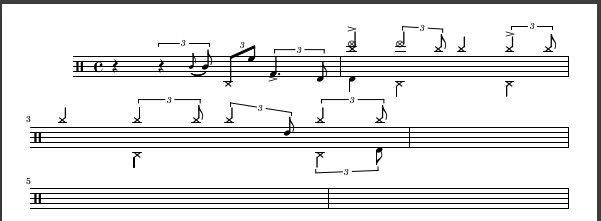
\includegraphics[height=50mm, width=160mm]{z_images/3_experimentations/experience_2/partition.png}\\\\
\textit{En cours…}
\newpage
\subsection{squant : parsing du fichier midi}
squant lit le midi\\
grammaire wta qui détermine le poid\\
La distance est automatiquement déterminée par squant\\
distance à l’input\\
complexité de la notation

On veut minimiser le coût et la distance $\Rightarrow$ Trouver un compromis.

./build/squant2 -h

Essayer le lire un fichier midi avec squant2
lire mesure par mesure
Regarder les wta(grammaire)

\subsubsection{Quelques tests de lecture midi}
\begin{verbatim}
Les 4 messages suivants sont présents dans tous les tests qui suivent :
[ info] schema file: test/schema/schema-01.wta (??? weight model option)
[warning] no declaration MAX\_GRACE in grammar file test/schema/schema-01.wta
[warning] no declaration TIMESIG in grammar file test/schema/schema-01.wta
[warning] MIDIfile has not joined tracks

./build/squant2 -v 4 -a test/schema/schema-01.wta -m 004_jazz-funk_116_beat_4-4.mid -config ./params.ini
[error] at least one of the options -bars or -barsec mandatory

./build/squant2 -verbosity 4 -schema test/schema/schema-01.wta -midi 004\_jazz-funk\_116\_beat\_4-4.mid -config ./params.ini -barsec 3

squant2: /home/martin/qparselib/src/schemata/SymbLabel.cpp:44: static label_t SymbLabel::make(unsigned char, SymbLabel::Kind, short unsigned int, short unsigned int): Assertion `info2 < 512' failed.
Abandon (core dumped)
\end{verbatim}

Tester squant2 avec le fichiers midi du corpus du gitlab\\\\

La commande suivante :
\begin{verbatim}
	build/squant2 -v 5 -a ./test/schema/schema-03-R.wta -m ~/corpus-master_qparselib/103-SaintSaens-elephant/perf/103_FJ.mid -config ./params.ini -mono -barsec 3.0 -ts 3/4	
\end{verbatim}

Donne :\\
(1) 3($\bullet$, $\overline{2}$:2($\bullet$, ), )\\
(2) 3($\bullet$, $\overline{2}$:2($\bullet$, $\bullet$), )\\
(3) 3($\bullet$, $\overline{2}$:2($\bullet$, $\circ$), )\\\\

% Reste de l’arbre avec des caractères pas encore fonctionnels :
%(4) 3(2̅(2̅(2̅(●, ●), ⏑), ⏑), ⏑:2, )
%(5) 3(2̅(2̅(●, ○), ●), ●:2, )
%(6) 3(2̅(●, 2̅(●, 2̅(○, ●))), ⏑:2, )
%(7) 3(2̅(●, ●), ●:2, )
%(8) 3(2̅(●, 2̅(●, 2̅(⏑, ●))), 2̅(⏑, 2̅(●, ○)), ●)
%(9) 3(●, ●:2, )
%(10) 3(●, 2̅:2(●, 2̅(●, 2̅(⏑, ●))), )
%(11) 3(⏑, 2̅:2(●, ○), )
%(12) 3(●, ⏑, ●)
%(13) 3(●, 2̅:2(2̅(●, 2̅(○, ●)), 2̅(⏑, 2̅(○, ●))), )
%(14) 3(⏑, 2̅:2(●, 2̅(●, ○)), )
%(15) 3(●, ●:2, )
%(16) 3(●, ○:2, )

Pour comprendre les grammaires :\\
Regarder les fichiers wta commentés.\\
https://qparse.gitlabpages.inria.fr/docs/scientific/\\
A\_Parse-based\_Framework\_for\_Coupled\_RhythmQuantization\_and\_Score\_Structuring.pdf
Réfléchir au coût de notation (grace notes, etc.)
\newpage

\subsubsection{cluster.md}
%https://gitlab.inria.fr/qparse/qparselib/-/blob/distance/notes/clusters.md\\\\

\textbf{Caroms of input events}\\

Carom is a synonym for « pileup ». An alternative term could be « cluster » (in the Musical sense, not in the ML sense!).\\

----------------------------------------------------------\\

\textbf{input segment}\\

we assume given in input a sequence of MIDI events $e_0, \ldots, e_n$​​ called "input segment".\\

Every input event is $e_i$ is made of :
\begin{itemize}
	\item an `ON`/`OFF` flag
	\item a MIDI pitch value in $0..127$​
	\item a MIDI velocity value in $0..127$
	\item a date in Real Time Unit (RTU) = seconds, or equivalently MIDI ticks.\\
\end{itemize}

The input events are time-increasing:
$$ date(e_0) \leq  date(e_1) \leq \ldots \leq date(e_n)$$

\textbf{attention:} input event $\neq$​ note (in score):

One input event may have different roles wrt the output score:
\begin{itemize}
	\item begining of note
	\item grace note
	\item trill
	\item end of note
	\item rest
	\item just ignored.\\e.g. in general in MIDI drum input, the `OFF` events will be ignored, but not for piano input.\\
\end{itemize}

----------------------------------------------------------\\

\textbf{Parsing}\\

During parsing, we try several alignements of the input events to particular points in the timeline.\\
The points for alignement are defined by time division, according to a derivation (parse tree) for a CF grammar (actually a tree in a regular tree grammar language).\\

The temporal alignment of an event is done to the point that is the closest to the date of event.
This way, it may happen that several events are aligned to the same point.\\
\newpage

----------------------------------------------------------\\

\textbf{Carom}\\

A carom is a sequence $e_i,\ldots, e_{i+k}$​​ of successive input events (\textit{i.e} a subsequence of the input segment), that ought to be aligned to the same time point. In practice, it is defined by the input segment, $i$ and $k$.\\

Intuitively, it means that the corresponding notes (or rests) will be simultaneous in the output score (e.g. notes in chords, or in different polyphonic voices), or that they will be grace notes.\\

Formally, we define for every transcription case (monophonic instrument, drum, guitar, piano...) a function that depends on the that takes in input\\
\begin{itemize}
	\item a carom $C = e_i,\ldots, e_{i+k}$,
	\item an index $0 \leq j \leq k$,\\
\end{itemize}


and returns the \textit{role} the input event  $e_{i+j}$ in $C$, among:\\
\begin{itemize}
	\item `Ignored`,
	\item `Note`,
	\item `Rest`,
	\item `Staccato`,
	\item `GraceNote`,
	\item `GraceRest`,
	\item maybe more to come...\\
\end{itemize}

For instance, in the case of drum transcription, all `OFF` events are ignored.\\

\textbf{Example 1:}\\\\
In the case of \textbf{drum} transcription, all the pitchs of the following events correspond to the snare-drum (sd).

\begin{table}[h]
\centering
\begin{tabular}{|c|c|c|c|c|}\hline
	event & $e_1$ & $e_2$ & $e_3$ & $e_4$ \\ \hline
	flag & ON & OFF & ON & OFF \\
	pitch & 38 & 38 & 38 & 38 \\ \hline
\end{tabular}	
\end{table}

Therefore we have a sd "flam" (\url{https://en.wikipedia.org/wiki/Drum\_rudiment#Flam}), defined by the following roles:

\begin{table}[h]
	\centering
	\begin{tabular}{|c|c|c|c|c|}\hline
		event & $e_1$ & $e_2$ & $e_3$ & $e_4$ \\ \hline
		role  & GraceNote & Ignored & Note  & Ignored \\ \hline
	\end{tabular}	
\end{table}

We say that $e_3$ is the \textit{main note} associated to (or \textit{decorated by}) the grace note $e_1$.\\

When $e_{i+j}$​ is a grace note ('flam' in the case of drum), we assume moreover a second mapping, called \textit{main}, that associate to $j$​  the index in $[j+1, k]$​ of the corresponding main note.\\

Example 1': in the previous example, $main(1) = 3$.\\



\textbf{Example 2:}\\\\¨
In the case of **monophonic** transcription, the following events: 

| event | $e_1$ | $e_2$ | $e_3$ |
| :---: | :---: | :---: | :---: |
| flag  |  ON   |  OFF  |  ON   |
| pitch |  64   |  64   |  62   |

also correspond to a grace note followed by a note:



| event |   $e_1$   |  $e_2$  | $e_3$ |
| :---: | :-------: | :-----: | :---: |
| role  | GraceNote | Ignored | Note  |



Example 3: still in the case of **monophonic** transcription, for the following events: 

| event | $e_1$ | $e_2$ | $e_3$ |
| :---: | :---: | :---: | :---: |
| flag  |  ON   |  ON   |  OFF  |
| pitch |  64   |  62   |  64   |

we also have the same roles as in Ex.2:



| event |   $e_1$   | $e_2$ |  $e_3$  |
| :---: | :-------: | :---: | :-----: |
| role  | GraceNote | Note  | Ignored |

Indeed, we ignore that fact that the OFF $e_3$ happens  after the ON $e_2$ of next note (e.g. because of the end gesture of the player on the keyboard), because we are in the monophonic case. 



Note that here, we process directly the MIDI input. No pre-processing is assumed, e.g. for eliminating overlaps between the notes 64 and 62. Somehow, elimination of overlaps is ensured by the *role* function for the monophonic case.



Example 4: Back to the case of **drum** transcription, the pitch of $e_1$​​ and $e_2$​ below corresponds to a tom and the one of $e_3, e_4$​ to the sd.

|   event    | $e_1$ | $e_2$ | $e_3$ | $e_4$ |
| :--------: | :---: | :---: | :---: | :---: |
|    flag    |  ON   |  OFF  |  ON   |  OFF  |
|   pitch    |  48   |  48   |  38   |  38   |
| timestamps |  t\_1  |  t\_2  |  t\_3  |  t\_4  |

It could be interpreted either as two simultaneous tom and sd notes, or as a flam between the tom and the sd (the tom is the grace note, the sd the main note). We choose between the two cases according to the "On Tick" distance $t_3 - t_1$.
More precisely, we assume a threshold $\varepsilon$​ such that:

- if $t_3 - t_1 < \varepsilon$​​ then we have 2 simultaneous notes  ("polyphony", between tom and sd, written as a chord):

| event | $e_1$ |  $e_2$  | $e_3$ |  $e_4$  |
| :---: | :---: | :-----: | :---: | :-----: |
| role  | Note  | Ignored | Note  | Ignored |

- if $t_3 - t_1 ≥ \varepsilon$ then we have a flam between tom and sd (written as a grace note):

| event |   $e_1$   |  $e_2$  | $e_3$ |  $e_4$  |
| :---: | :-------: | :-----: | :---: | :-----: |
| role  | GraceNote | Ignored | Note  | Ignored |

The threshold $\varepsilon$ may depend on the latency of an electronic  (MIDI) drum kit used for recording, and/or neuro-acoustic features such as the duration between 2 percussive events above which the perception change from simultaneous, to the phoneme '*flam*'.


\subsubsection{Contributions}
Contribution sur la branch « distance » dans :\\
\begin{itemize}
	\item qparselib/notes/cluster.md
	\item qparselib/src/segment/import/ :\\
	      DrumCode hpp et cpp\\
\end{itemize}
\newpage
\section{Conclusion}
Conclusion de ce chapitre.


%%%%%%%%%%%%%%%%%%%%%%%%%%%%%%%%%%%%%%%%%%%%%%%%%%%%%%
%% RÉSULTATS
%%%%%%%%%%%%%%%%%%%%%%%%%%%%%%%%%%%%%%%%%%%%%%%%%%%%%%

\chapter{Résultats}
\label{chap:resultats}
\minitoc

\textit{\\Résultats (chapitre~\ref{chap:resultats})~: les résultats
obtenus sur chacune des expériences~;}

\section{Introduction}
Dans ce chapitre...

\section{Contenu}
Une section dans ce chapitre...

\section{Conclusion}
Conclusion de ce chapitre.


%%%%%%%%%%%%%%%%%%%%%%%%%%%%%%%%%%%%%%%%%%%%%%%%%%%%%%
%% DISCUSSION
%%%%%%%%%%%%%%%%%%%%%%%%%%%%%%%%%%%%%%%%%%%%%%%%%%%%%%

\chapter{Discussion}
\label{chap:discussion}
\minitoc

\textit{\\Discussion (chapitre~\ref{chap:discussion})~: la discussion des
résultats obtenus (quelle expérience a produit les meilleurs
résultats, de manière globale, dans le détail des catégories) avec,
si possible, une analyse des erreurs pour comprendre les
possibilités d'amélioration~;}

\section{Introduction}
Dans ce chapitre...

\section{Contenu}
Une section dans ce chapitre...

\section{Conclusion}
Conclusion de ce chapitre.


%%%%%%%%%%%%%%%%%%%%%%%%%%%%%%%%%%%%%%%%%%%%%%%%%%%%%%
%% CONCLUSION
%%%%%%%%%%%%%%%%%%%%%%%%%%%%%%%%%%%%%%%%%%%%%%%%%%%%%%

\cleardoublepage\pdfbookmark[-1]{Conclusion générale}{conclusion} %% CG: lien dans le PDF hors d'une partie
\chapter*{Conclusion générale}
\adjustmtc
\addstarredchapter{Conclusion générale}
\textit{\\Conclusion~: la conclusion globale du mémoire.}\\\\
Dans ce mémoire, nous avons traité de la problématique...\\\\
Dans ce mémoire, nous avons traité de la problématique de la transcription automatique de la batterie. Son objectif était de transcrire, à partir de leur représentation symbolique MIDI, des performances de batteur de différents niveaux et dans différents styles en partitions écrites.\\
Nous avons avancé sur le parsing des données MIDI établissant un processus de regroupement des évènements MIDI qui nous a permis de faire la transition du monophonique vers le polyphonique. Une des données importante de ce processus était de différencier les nature des notes d’un \textit{accord}, notamment de distinguer lorsque 2 notes constituent un \textit{accord} ou un \textit{fla}.\\
Nous avons établis des \textit{grammaires pondérées} pour le parsing qui correspondent respectivement à des métriques spécifiques. Celles-ci étant sélectionnables en amont du parsing, soit par indication des noms des fichiers MIDI, soit par reconnaissance de la métrique avec une approche dictionnaire de patterns prédéfinis \footnote{\textit{Motifs} dans les \textit{systèmes} de la présente proposition.} qu’il serait pertinent de mettre en œuvre en machine learning.\\
Nous avons démontré que l’usage des \textit{systèmes} élimine un grand nombre de calcul lors de la réécriture. Pour la séparation des voix grâce au motif d’un système et pour la simplification grâce aux gammes du motif d’un système. Nous avons aussi montré comment, dans des travaux futurs, un système dont le motif serait reconnu en amont dans un fichier MIDI pourrait prédéfinir le choix d’une grammaire par la reconnaissance d’une métrique et ainsi améliorer le parsing et accélérer les choix ultérieurs dans la chaîne de traitement en terme de réécriture.\\
Il sera également intéressant d'étudier comment l'utilisation de LM peut améliorer les résultats de l'AM, voir [2], et ouvrir la voie à la génération entièrement automatisée de partitions de batterie et au problème général de l'AMT de bout en bout.\cite{future_directions}


% ================================== BIBLIOGRAPHIE =============================

\cleardoublepage\pdfbookmark[-1]{Bibliographie}{bibliography}
%\selectlanguage{english}
 
\bibliographystyle{unsrt} % Les entrées sont disposées selon leur ordre d’apparition dans la base de donnée bibliographique et étiquetées par un numéro entre crochets.
\bibliography{x_biblio} % pour afficher la biblio
%\selectlanguage{french} 

\appendix
\cleardoublepage\pdfbookmark[-1]{Annexes}{appendix}
%% TODO: mettre en commentaires les annexes, ou remplacer l'appel de
%% fichier *.tex par votre fichier d'annexe.
\include{z_annexe_lilypond}
%\documentclass{report}
\usepackage[pagebackref,colorlinks=true,citecolor=forestgreen,linkcolor=black,menucolor=alezan]{hyperref}
\begin{document}
\chapter{Principes à suivre}

\section{Le sujet de votre mémoire}
Vous avez acquis, au cours de l'année 2015-2016, des compétences d'ingénieur-linguiste ; vous savez donc analyser un problème, proposer une méthodologie permettant d'arriver à une solution et montrer les limites de cette dernière. C'est cette démarche qui constituera le fil directeur de votre mémoire.

Ce travail devra être original et personnel. Le cadre de votre travail est naturellement la linguistique et, étant donné le diplôme que vous préparez, la linguistique appliquée, plutôt que théorique. Ceci ne veut néanmoins pas dire que vous ne devrez pas situer votre démarche à l'intérieur d'un cadre théorique, au contraire. On souhaite cependant que ce cadre serve d'appui à la création ou à la transformation d'outils, à la mise au point de méthodologies vous permettant de proposer un résultat.

Cela revient à dire que votre mémoire constitue une tentative de problématiser une approche méthodologique, de proposer une piste nouvelle, de comparer des méthodes, des outils, etc. Il contiendra en tout cas un état de l'art et s'appuiera sur une bibliographie précise et récente. L'état de l'art ne doit pas être déconnecté de la question traitée : on ne vous demande pas de faire un état de l'art pour faire un état de l'art mais, au contraire, de montrer comment se situe votre travail par rapport à cet état de l'art.
Si votre sujet s'y prête, et afin d'en faciliter la réalisation, vous pouvez segmenter votre état de l'art en plusieurs parties ciblées à placer en tête des chapitres correspondant plutôt que d'écrire un chapitre consacré qui risque d'être généraliste et donc insuffisamment précis.

Vous devrez avoir choisi un sujet de mémoire à la mi-mai ou, à tout le moins, avoir réfléchi à des pistes sérieuses. Vous devrez vous assurer auprès d'un intervenant du TIM/ER-TIM que vous ne faites pas fausse route et que votre mémoire ne sera pas hors-sujet. Il s'agit d'éviter que vous ne traitiez un sujet dont les exigences techniques pourraient s'avérer supérieures à ce que vous croyez connaître. Le(s) stage(s) de fin d'études que vous devez entreprendre peu(t/vent) vous aider à affiner votre choix de sujet, mais vous devez garder à l'esprit que votre mémoire ne doit pas se confondre avec une description de votre stage. Notez bien que les rapports de stage ne sont pas pris en compte dans l'évaluation de votre Master.

Pour vous aider, vous pouvez consulter les meilleurs mémoires des années précédentes (et dont les résumés sont en ligne sur le site \url{www.er-tim.fr}). \'Evidemment, vous consulterez également les articles scientifiques liés à votre problématique : outre les connaissances que vous pourrez ainsi acquérir, cela vous permettra aussi de vous familiariser avec ce genre bien spécifique. Si vous ne trouviez pas de sujet vous permettant de mettre en pratique les connaissances acquises au cours de cette année, en fonction de vos goûts et attentes personnels ou professionnels, nous vous en proposerions un (consultez-nous, donc).

\section{L'encadrement du mémoire}
Vous avez toute latitude pour choisir, selon affinités, la/les personne(s) qui va/vont diriger vos recherches. Mais un/des intervenant(s) du TIM/ER-TIM figurera/ont nécessairement dans votre jury lors de la soutenance. Il faut donc nécessairement avoir pris contact avec ces personnes et s'assurer de leur collaboration. Si vous envisagez de faire une thèse ensuite, il est recommandé de solliciter un enseignant assimilé professeur ou habilité à diriger des recherches ou de mettre en place un co-encadrement en ce sens.

En règle générale, le TIM/ER-TIM souhaite, autant que faire se peut, que les personnes qui vous ont encadré lors de votre stage et qui ont pu vous conseiller pour la rédaction de votre mémoire, soient présentes lors de la soutenance. Elles apportent un complément d'information interne sur le stage et les conditions de réalisation du mémoire, éclairage qui peut être tout à fait pertinent.

Si vous rencontrez des problèmes et souhaitez poser des questions, il est impératif, dans un premier temps, de les formuler par courrier électronique plutôt que de venir immédiatement au TIM/ER-TIM, riche en compétences mais pauvre en personnel. Par ailleurs, vous ne devez pas envoyer par courrier électronique des centaines de pages à fin de re-lecture : lorsqu'une pré-version de votre travail vous semblera digne de relecture, déposez-la au TIM/ER-TIM, ou postez-la.

\section{L'évaluation du mémoire}
L'évaluation du mémoire est fonction de la qualité de votre travail écrit et de votre capacité à répondre aux questions, remarques, critiques qui peuvent vous être adressées pendant la soutenance. La qualité du travail écrit dépend de plusieurs critères, dont voici une liste non-exhaustive :
\begin{itemize}
\item votre mémoire forme-t-il un ensemble cohérent qui doit son unité à la volonté de répondre à une problématique bien définie ?
\item votre mémoire est-il réutilisable par une personne souhaitant faire un bilan de la problématique soulevée, tant du point de vue fond que forme (clarté de la bibliographie, description en annexe des outils utilisés avec liens aux sources, disponibilités des sources sur le CD-ROM d'accompagnement de votre mémoire, index permettant une consultation rapide, table des matières, pagination, etc.) ?
\item votre mémoire répond-t-il vraiment à l'objectif fixé au départ ? le titre de votre mémoire correspond-il vraiment au contenu ? les mots-clés qui seront mis en ligne sont-ils pertinents ?
\item votre mémoire met-il en valeur un angle de vue original sur un savoir-faire classique ?
\item votre mémoire parvient-il à mettre la théorie à l'épreuve ? \^Etes-vous capable de fournir des résultats, des exemples, un bilan d'expérience, des critères d'évaluation, une évaluation ?
\item la bibliographie doit être totalement normalisée, de façon à permettre une consultation aisée, les annexes contiendront un descriptif pratique et les références des outils utilisés, un échantillon des corpus utilisés et des programmes que vous avez écrits et, de manière générale, tout ce qui peut illustrer le travail réalisé. Attention, pour des raisons de place, vous ne devez évidemment pas présenter tous vos corpus et tous vos programmes en annexe, mais un simple échantillon. En revanche, corpus\footnote{Vérifiez toutefois que vous avez le droit de reproduire tout ou partie du corpus sur lequel vous aurez travaillé, en particulier pour les corpus de documents cliniques.} et programmes figureront impérativement et exhaustivement sur le CD fourni.
\end{itemize}

La qualité de votre prestation orale est importante. Vous devrez vous assurer, en particulier, que :
\begin{itemize}
\item vous savez vous affranchir du plan de votre mémoire mais vous devez néanmoins faire un bref résumé de la problématique car tous les membres du jury n'auront pas lu votre mémoire
\item vous donnez des exemples concrets des questions qui se sont posées et des solutions apportées, de façon à montrer que vous ne traitez pas le sujet de façon purement théorique
\item vous savez situer la problématique de votre mémoire par rapport aux travaux les plus connus et les plus récents sur la question
\item vous savez faire le lien entre les connaissances acquises au cours de l'année et la mise en pratique de ces connaissances lors de la réalisation du mémoire
\item vous savez répondre aux questions ou critiques qui vous sont soumises
\end{itemize}

\section{La démarche à suivre pour soutenir}
Trois semaines avant la date de soutenance, vous devez envoyer une version présentable de votre mémoire à votre encadrant et à l'équipe de formation, pour déterminer si le mémoire est soutenable. Vous devez remettre une version papier définitive de vos mémoires au moins 15 jours avant la soutenance.
\begin{itemize}
\item La soutenance pour la première session est fixée entre le 20 et le 24 juin 2016 (à préciser) pour ceux d'entre vous qui candidateraient à un contrat doctoral INaLCO (voir la procédure sur le site \url{www.inalco.fr}, le comité de sélection ayant lieu le 1 juillet 2016).
\item Pour la deuxième session (inscription en doctorat à l'INaLCO selon la procédure normale), la soutenance est fixée le 30 septembre 2016.
\item Pour la dernière session, la date de soutenance est fixée le 18 novembre 2016.
\end{itemize}

Vous devez déposer votre travail au moins deux semaines avant d'espérer soutenir. Il faut en effet qu'il soit lu, puis, si nécessaire, amendé et corrigé -- voire rejeté et réécrit -- de façon que la soutenance ne verse pas dans la critique systématique.

Au plus tard la veille de votre soutenance, vous aurez envoyé à \url{crim@inalco.fr} et à \url{sophie.urbaniak@inalco.fr} un résumé de votre mémoire de 10 lignes maximum ainsi que 5 mots-clés permettant de situer votre travail. Attention, ces informations sont destinées à être consultées et doivent donc être le reflet fidèle de votre travail final.

Une fois votre travail accepté, nous vous proposerons un ordre de passage pour la soutenance. Vous devrez fournir 3 exemplaires/support-papier et 3 exemplaires/support-électronique de votre mémoire (ces exemplaires sont destinés aux membres du jury et aux futurs étudiants). Sur le 4ème de couverture vous agraferez une enveloppe format 21-27 qui contiendra le CD correspondant à votre travail. Ce CD contiendra, outre la version électronique de votre mémoire, toutes les annexes ne pouvant figurer dans le mémoire pour des raisons de place : corpus, code source des outils utilisés, polices de caractères utilisées, code des programmes que vous avez élaborés.
\end{document}


% =============================== INDEX DES NOTATIONS ==========================

\cleardoublepage % pour forcer l'index à apparaître sur une page impaire
\pdfbookmark[-1]{Index}{index}
\printindex % pour afficher l'index

%% \newpage
%% \thispagestyle{empty}
%% \mbox{}

\end{document}
